\documentclass [12pt,letterpaper]{report}

% Standard packages
\usepackage{amsmath}		% Extra math definitions
\usepackage{graphics}		% PostScript figures
\usepackage{setspace}		% 1.5 spacing
\usepackage{longtable}          	% Tables spanning pages
\usepackage{subfig}
\usepackage[ampersand]{easylist}

% Aaron's Packages
\usepackage{Style/ichago}   % The ichago references style
\usepackage{url}            % For formatting urls
\usepackage{listings}       % For formatting code
\usepackage{color}
\usepackage{sidecap}
\usepackage{wrapfig}
\usepackage{pgfplots}

\pgfplotsset{my style/.append style={axis x line=middle, axis y line=middle, xlabel={$x$}, ylabel={$y$}, axis equal }}

\definecolor{dkgreen}{rgb}{0,0.6,0}
\definecolor{gray}{rgb}{0.5,0.5,0.5}
\definecolor{mauve}{rgb}{0.58,0,0.82}

\lstset{frame=tb,
  language=C,
  aboveskip=3mm,
  belowskip=3mm,
  showstringspaces=false,
  columns=flexible,
  basicstyle={\small\ttfamily},
  numbers=none,
  numberstyle=\tiny\color{gray},
  keywordstyle=\color{blue},
  commentstyle=\color{dkgreen},
  stringstyle=\color{mauve},
  breaklines=false,
  breakatwhitespace=false,
  frame = single,
  lineskip = 0pt,
  tabsize=3
}

% Custom packages
\usepackage[first]{Style/datestamp}			% Datestamp on first page of each chapter
\usepackage[fancyhdr]{Style/McECEThesis}	% Thesis style
\usepackage{Style/McGillLogo}			% McGill University crest

% $Id: ThesisEx.tex,v 1.1 2005/06/09 12:48:46 kabal Exp $

\usepackage{color}
\def\headrulehook{\color{red}}		% Color the header rule

%===== page layout
% Define the side margins for a right-side page
\insidemargin = 1.3in
\outsidemargin = 0.8in

% Above margin is space above the header
% Below margin is space below footer
\abovemargin = 1.1in
\belowmargin = 0.75in

%========= Document start

\begin {document}

%===== Title page

\title{A Flexible Tool for the Visualization and Manipulation of Musical Mapping Networks}
\author{Aaron Henry Krajeski}
\date{\Month\ \number\year}
\organization{%
    \\[0.2in]
    \McGillCrest {!}{1in}\\	% McGill University crest
    \\[0.1in]
    Department of Music Technology\\
    Schulich School of Music, McGill University\\
    Montreal, Canada}
\note{%
    {\color{red} \hrule height 0.4ex}
    \vskip 3ex
    A thesis submitted to McGill University in partial fulfillment of the
    requirements for the degree of Master of Arts.
    \vskip 3ex
    \copyright\ \the\year\ Aaron Henry Krajeski
}

\maketitle

%===== Justification, spacing for the main text
\raggedbottom
\onehalfspacing
\pagenumbering{roman}

%===== Abstract, Sommaire & Acknowledgments
\section*{\centering Abstract}

This report describes the use of \LaTeX{} to format a thesis.
A number of topics are covered: content and organization of the thesis,
 \LaTeX{} macros for controlling the thesis layout, formatting mathematical
 expressions, generating bibliographic references, importing figures and
 graphs, generating graphs in {\small MATLAB}, and formatting tables.
The \LaTeX{} macros used to format a thesis (and this document) are
 described.

\newpage

\section*{\centering Acknowledgments}
Acknowledge this, asshole.
\pagebreak

\section*{Preface}

There are some things I should probably pre-face, certainly not reface.
%Thesis regulations require that contributions by others in the collection of materials and data, the design and construction of apparatus, the performance of experiments, the analysis of data, and the preparation of the thesis be acknowledged.
\pagebreak

%========== Tables of contents, figures, tables
\tableofcontents
\listoffigures
	various graphs of response time (discussion)
	screenshot of drawing
	screenshot of saving/loading
	screenshot of main view
	screenshot of grid view
\listoftables

\newpage
\chapter*{List of Acronyms}\markright{List of Terms}

\begin{longtable}{ll}
    DMI 	& 	Digital Musical Instrument\\
    GUI		& 	Graphical User Interface\\
    IDMIL &   Input Devices for Musical Interaction Laboratory\\ 
    API   &   Application Programming Interface\\
    SWIG  &   Simplified Wrapper and Interface Generator\\
    OSC   &   Open Sound Control\\
    MVC   &   Model View Controller\\
    HTTP  &   HypterText Transfer Protocol\\
    HTML  &   HyperText Markup Language\\
    CSS   &   Cascading Style Sheet\\
     %URL ?
\end{longtable}

\cleardoublepage
\pagenumbering{arabic}

%%========== Chapters
%\typeout{}
%\chapter{Introduction \& Motivation}

\section{Why Develop the Use of Sonification for Affective Computing?}
In this section I will talk about why we should try to develop sonification strategies for affective display

\begin{enumerate}
\item Use when visual or verbal attention is already occupied:
	\begin{enumerate}
	\item When interacting with a visual interface
	\item When interacting with another human
	\end{enumerate}
\item Use to show bodily-based measures of affect that are not socially communicated (e.g. Electrodermal Activity)
\item Emotional Communication benefits from diversity and redundancy (best to have as many cues as possible for conveying emotion)
\item There is a need for continuous display of arousal and valence (that is, there are technologies that can produce continuous display of arousal and valence).
\item Non-speech audio seems remarkably capable of emotional communication using simple psychoacoustic cues
\end{enumerate}

\subsection{When Visual or Verbal Attention is already occupied}
\section{Affective Display}

In the literature on affective computing, most articles are written on emotion recognition or modelling.  Technologies for displaying emotional information or mediating emotional communication however are very important as they form the basis of meaningful communication with the human agent.  There are many ways of displaying emotional information.  Popular and well-researched methods use facial display, gesture or postural display, or speech prosody.  These are very effective mechanisms and highly useful.  

One disadvantage of these is that they require visual or verbal attention, so in situations where visual or verbal attention is already occupied, their use adds significantly to the cognitive load.  Another related limitation is their requirements for display.  For instance, displaying synthesized faces or gestures to communicate emotion require a visual monitor or in the case of robotics, a face or a robotic-body.  In the case of using speech for emotional communication, there is a requirement of a voice or speech for transmission.  When their is no linguistic content to be conveyed, synthesized speech is not useful.

The benefits of sound is that it can be used to monitor emotions in an eyes and speech-free fashion.  Using sound, one can use the eyes to simultaneously interact with a user interface or another human.  Similarly, one can listen to another human speaking while still being able to monitor emotions. 

\section{Why Use ``Emotional" Sounds instead of Abstract Sounds? (Sonification, Auditory Icons or Earcons?)}

In sonification, often there is no clear correspondence between data and sound a priori, so an important part of the mapping is creating a metaphor that can be quickly understood by the listener but also used to hear out subtle details so that it can be used as a data bearing medium.  The problem when using sonification for display of arousal and valence, as is being discussed presently, is that the underlying data may be more accurately presented using a mapping that \textit{doesn't} use emotional cues.  Furthermore, another mapping strategy may create a more convincing metaphor  (Give an example, maybe a hammer on a piece of wood).  So why use psychoacoustic cues determined by emotional studies?

\begin{description}
\item[Clear mappi	ng/universality] One doesn't need to explain what to listen for in the mapping.  A sound just is "happy" or "sad."
\item[``Low-Level Processing"] Just as you can listen to music in a movie and have it influence your emotions w/o having to pay attention, a sonification mapping strategy consistent w/ these cues can be analyzed on a lower level.
\item[Applies Experimental Predictions] Although there is a vast literature on auditory perception, parameter mapping sonification often applies complex auditory models for data display, each context applying different models, and in general there is no consensus on the best way to do mapping, though many ways have been proposed.  Unlike in most cases, the literature on the psychoacoustic elicitors of emotion is huge and goes back three-quarters of a century.  Further, there are now computational models that predict listeners responses to music from these low-level features (Cite Coutinho 2009).  It just makes sense to draw from a literature that is already so huge.
\item[Contributes to Emotion Research]  Developing these sorts of models provides music researchers with acoustic models that use the features they predict to convey emotion, but do not have the associations with music that music has.  Therefore, it would be reasonably impossible for a listener to ``recognize" a sonification as they could recognize a piece of music.  Therefore this sort of emotional induction would be impossible.  Same thing with Juslin's other non-acoustic mechanisms.  Abstracting into a range of just psychoacoustic features provides a level of ``cleanness" to experimental stimuli.    


\end{description}


%\section{Affective Computing}

%\section{Problem Statement}

%\section{Contributions}

%\section{Thesis Overview}



































%
\typeout{}
%!TEX root = ../thesis.tex

\chapter{Introduction \& Motivation}
%%%%%%%%%%%%
%  (start with some kind of epigraph, maybe Tufte?)
%  cite: maybe Marcelo's paper on mapping, DOT, libmapper
%	look at Joe's 1-3
%	1: separate parts
%	S. Mann, “Natural interfaces for musical expression: Physiphones and a physics-based organology,” in Proceedings of the 2007 Conference on New Interfaces for Musical Expression (NIME-07), (New York, USA), pp. 118–123, 2007.
%	2: controller any arbitrary shape
%	E. R. Miranda and M. M. Wanderley, New Digital Instruments: Control and Interaction Beyond the Keyboard, vol. 21 of The Computer Music and Digital Audio Series. Middleton, Wisconsin, USA: A-R Editions, Inc., 2006.
%	3: mapping
%	J. Ryan, “Some remarks on musical instrument design at STEIM,” Contemporary Music Review, vol. 6, no. 1, pp. 3–17, 1991.
%	probably use marcelo's paper instead
%%%%%%%%%%%%

\begin{quote}
``In order that our tools, and their uses, develop effectively: (A) we shall have to give still more attention to doing the approximately right, rather than the exactly wrong...'' \cite{tuckey}
\end{quote}

Throughout the vast majority of human history the term ``musical instrument'' has signified both the physical object with which the musician interacted \emph{and} the direct source of the sound created: a violin with vibrating strings, a reeded saxophone, a timpani with its membrane, etc.  With the advent of electronic sound in the late 19\textsuperscript{th} century, it became possible for interactive objects to be separated from the sound producing devices they control \cite{chadabe}.
As technological development progressed, so did the capacity to divide musical instruments into independent parts. With digitization it is now not only possible to arbitrarily connect a control element to any sound synthesis dimension, but also to modify this association according to the whims of the user. Since mechanical linkages are no longer necessary in the design of musical instruments, control surfaces can, and often do, take on a variety of wild and arbitrary shapes and modes of interaction.\footnote{International Conference on New Interfaces for Musical Expression. [Online]. Available: \url{http://www.nime.org/}. Accessed June 23, 2013.}
All that is necessary for this process is for control devices to output some kind of electronic signal that other, sound-producing instruments can accept. With no obvious means of implementation, the success or failure of these new digital musical instruments (DMIs) often depends on how artfully their output signals are ``mapped" to synthesis parameters.

More and more frequently, the mapping itself becomes a part of the expressive element of a musical work \shortcite{mappingstrategies},
as it associates itself with both composition and performance with certain DMIs. Thus is becomes necessary for mapping to be dynamic and interactive: sometimes poured over in composition studios, or sometimes edited mid-piece. Musicians are not necessarily computer programmers, thus ideally the act of mapping should not require computer expertise. This means that on top of the low-level layer of interactive mapping (simply instructing a machine to connect signals to others in specific ways), there needs to exist an interface to make such an activity easy, logical, intuitive and in line with the artistic process.

As the actual act of mapping is as expansive and nebulous as the instruments it hopes to assist, thus the design of such a mapping interface presents many interesting challenges. Due to the tremendously wide variety of possible use cases, several seemingly contradictory goals emerge: What is the best way to visually represent complex musical networks while simultaneously allowing for the user to easily manipulate them? How can systems with many devices and signals be well represented while still allowing in-depth control of small networks? How can an interface be transparent to non-technical users while still accommodating all possible functionality that advanced users may wish to use? 

%Though it may not be possible to find a perfect solution to all of the above questions, it \emph{is} feasible address each in turn and accept the best available compromise. Overall it is simply necessary to wonder: What are useful features of a graphical interface for musical mapping?

\section{Context and Motivation}

The world of digital musical instruments is still dominated by keyboard type input devices. Though many novel DMIs currently exist (and many more are being created) these devices are usually unique and often difficult to use without their creator being present \cite{squeezevox}.
Since mapping is such an important feature of DMIs, a means of transparently editing them could inspire more people to use novel musical controllers. In response to this challenge, libmapper, a tool for collaborative mapping, was created at the Input Devices and Music Interaction Laboratory (IDMIL).

In its most basic state, libmapper takes the form of an application programming interface (API). APIs are primarily a means for different pieces of computer software to communicate with one another. The only possible way to communicate directly with the libmapper API is through coded text. For example, figure \ref{fig:libmapper_code} causes a synthesizer to announce itself and begin communicating with other devices on a libmapper-enabled network \shortcite{malloch}.

\begin{figure}[h!]
\begin{lstlisting}[]
#include <mapper.h>
mapper_admin_init();
my_admin = mapper_admin_new("tester", MAPPER_DEVICE_SYNTH, 8000); 
mapper_admin_input_add(my_admin, "/test/input","i")) 
mapper_admin_input_add(my_admin, "/test/another_input","f"))

// Loop until port and identifier ordinal are allocated. 
while ( !my_admin->port.locked	|| !my_admin->ordinal.locked )
{
	usleep(10000); // wait 10 ms 
	mapper_admin_poll(my_admin);
}

for (;;) 
{
	usleep(10000);
	mapper_admin_poll(my_admin); 
}
\end{lstlisting}
\caption{A sample of libmapper code}
\label{fig:libmapper_code}
\end{figure}

This is obviously inaccessible to users who do not have the time or desire to read through documentation files, or those who have no knowledge of programming semantics. A steep learning curve is especially a problem for a network tool like libmapper: because it is primarily a means of communication between instruments, it can only be successful if it is widely adopted. A libmapper-enabled controller will only be useful if many high quality libmapper synthesizers exist. In turn, synthesizer makers will only have incentive to incorporate libmapper into their designs if there are already controllers that use the system. 

An API can be contrasted with a graphical user interface (GUI), an interface that contains abstractions on top of the raw code. These abstractions can be features like buttons, menus, visual representations of data, etc. In general, GUIs are designed to be familiar to those who have used digital devices in the past, and thus easy to learn and use. Two GUIs have been created for libmapper (see section \ref{sec:priorGUIs}): a basic interface built in Max/MSP\footnote{MAX: You make the machine that makes your music. [Online]. Available: \url{http://cycling74.com/}. Accessed June 17, 2013} and vizmapper \cite{vizmapper}, a more abstract representation of a libmapper network. Both of these GUIs have their strengths, yet neither adequately meets the full range of possible use cases for libmapper. A more flexible approach is required if the GUI is to be usable in situations with hundreds of signals, transparent for systems with multi-leveled hierarchical devices, intuitive during performances where devices output light and haptic feedback as well as sound, and responsive for tasks where speed of manipulation is an absolutely necessity. 

With such an interface in place, libmapper can greatly expand its user base. As a result, more controller and synthesizer designers may choose to incorporate libmapper into their devices, and in turn these devices will be easier to learn and use. Hopefully the end result will be greater adoption of non keyboard-based DMIs in the electronic music community.

%Possible use cases: Performance, composition, demonstration (of a new DMI), experimentation
%	Actuator need not necessarily to be SOUND devices, but could be vibrotactile feedback, light projectors, 

\section{Project Overview}

The focus of this project is to create a graphical user interface for libmapper. This interface aims to be flexible and intuitive, simultaneously allowing for useful control of the full range of possible libmapper networks while also not intimidating non-technical users with complexity. The presupposed solution to this problem is to provide users with multiple independent modes of viewing and interacting with the network. Certain view modes can excel in providing precise control, while others can help users understand the structure of complex networks. The idea is to provide multiple imperfect solutions to an unsolvable problem, so that each can be ``...approximately right, rather than exactly wrong'' \shortciteA{tuckey}.

This project was structured in four major, non-sequential parts: a review of prior visualized mapping interfaces, the integration of presently available GUIs for libmapper, the extension of interface features and the collection of user feedback. Results of the research phase informed implementation and are presented here. Development began by updating a cross-platform implementation of the current Max/MSP-based GUI, while integrating functionality from vizmapper. New view modes were integrated into design while refining functionality of the previous ones. Throughout the design process, the GUI was provided to potential users who gave feedback on the strengths, weaknesses and potential avenues for improvement.

\section{Thesis Overview}

The remainder of this document is organized as follows. Chapter 2 outlines concepts necessary for providing context for this thesis project. A wide variety of domains inform the creation of a musical mapping interface. Special attention is paid to mapping theory, data visualization, relevant existing user interfaces, user centric design techniques and specifics of libmapper itself. Chapter 3 describes the design and implementation of the libmapperGUI. This chapter presents design decisions made, technical details of implementation and how the user-centric approach informed the process. Chapter 4 evaluates results, both on the empirical level of software performance as well as qualitative user feedback. Finally, Chapter 5 presents conclusions of the work and suggests further developments for the software.

\section{Contributions}

The contributions of this thesis are: the exploration of issues related to user interface design for musical mapping networks, the design and implementation of an interface for libmapper that aims to improve on usability and flexibility of the system, and this thesis document, which describes the research and development therein.


%
\typeout{}
%!TEX root = ../thesis.tex
\chapter{Background}

Dynamic mapping is becoming an increasingly important requirement for digital musical instruments. This chapter surveys currently available tools that allow for manipulation of musical and non-musical networks in real time. The first section presents a review of mapping itself, both from a theoretical and a musical standpoint. This portion also introduces the libmapper application programming interface. The second section reviews relevant work in the visual representation of information. The following portion describes applicable techniques in user interface design. Finally, a review of user interfaces for mapping is presented.

%%%%%%%%%%%%%%%%%%%%%%%%%%%%%%%%%%%%%%%%%%%%%%%%%%%%%%%%%%%%%%%%%%%%%%%%%%%%%%%%%%%%%%%%%%%%%%%%%%%%%%%%%%%%%%%%%%%%%%%%%%%%%%%%%%%%%%%%%%%%%%%%%%%%%%%%%%%%%%%%%%%%%%%%%%%%%%%%%%%%%%%%%%%%%%%%%%%%%%%%%%%%%%%%%%%%%%%%%%%%%%%%%%%%%%%%%%%%%%%%%%%%%%%%%%%%%%%%%%%%%%%%%%%%%%%%%%%%%%%%%%%%%%%%%%%%
\section{Mapping}

At the most fundamental level, \emph{mapping} is the act of associating two or more sets of information. Mappings can be mathematical, computational, linguistic (like translation), geographic, or even poetic\footnote{What is metaphor if not the association of unlike things?}. Within the context of DMI design mapping is the relationship between sensor outputs and synthesis inputs. The entire character of a new instrument can be drastically altered though mapping, even while control surface and sound source are held constant \shortcite{hunt_mapping_is_important}. As a result, the theoretical formalism of mapping becomes yet another necessary tool in the modern instrument designer's arsenal.

%%%%%%%%%%%%%%%%%%%%%%%%%%%%%%%%%%%%%%%%%%%%%%%%%%%%%%%%%%%%%%%%%%%%%%%%%%%%%%%%%%%%%%%%%%%%%%%%%%%%%%%%%%%%%%%%%%%%%%%%%%%%%%%%%%%%%%%%%%%%%%%%%%
\subsection{Mapping Theory}

	\subsubsection{Mapping as function and mapping cardinality}
	\label{sec:mapping_classes}

From the perspective of mathematics, the term \emph{mapping} is very nearly synonymous with \emph{function} \cite{native_set_theory}, as both describe how one set of numbers corresponds with another. The first group is commonly referred to as the \emph{domain} and the second as the \emph{codomain} or \emph{range}. An in-depth review of functions in mathematics is beyond the scope of this thesis, however a few fundamental examples will be useful for reference in section \ref{sec:mappingforDMIs}. The following are instances of two basic types of mathematical functions:

\begin{equation} y = 2x - 1 \label{eq:one-to-one} \end{equation} 
\begin{equation} y = x^2  \label{eq:many-to-one}  \end{equation}

Each function takes a single input value (\emph{x}) and \emph{maps} that number onto its range (\emph{y}). 
%For example, an input of \textbf{5} maps to \textbf{9} in equation \ref{eq:one-to-one}, while the same input results in an output \textbf{25} for equation \ref{eq:one-to-many}. 
The fact that each of these equations take in only a single number as input, and output a single number in turn, means they can be graphed in a two dimensional space. This is not necessarily the case, as functions can input and output lists of numbers (vectors). Mathematically they are not very interesting, but they represent two fundamentally different \emph{kinds} of functions.

\begin{figure}[h]
	\centering
	\begin{tikzpicture}
		\begin{axis}[my style, xtick={-2,-1,...,2}, ytick={-2,-1,...,2}, xmin=-2, xmax=2, ymin=-2, ymax=3]
			\addplot[domain=-100:100]{2*x-1}; 
		\end{axis}
	\end{tikzpicture}	
\caption{The function described in equation \ref{eq:one-to-one}, graphed in two dimensions.}
\label{fig:one-to-one_graph}
\end{figure}

For equation \ref{eq:one-to-one} each input value has \emph{one and only one} corresponding output value. The same is true if the function is to be inverted, as each output value corresponds to only one input value. The range is simply a scaled and shifted version of the domain. The mapping's \emph{one-to-one} nature can clearly be seen in figure \ref{fig:one-to-one_graph}. To mathematicians this is known as the mapping's \emph{cardinality}.

\begin{figure}[h]
	\centering
	\begin{tikzpicture}
		\begin{axis}[my style, xtick={-3,-2,...,3}, ytick={-3,-2,...,3}, xmin=-3, xmax=3, ymin=-1, ymax=4]
			\addplot[domain=-3:3]{x^2}; 
		\end{axis}
	\end{tikzpicture}
\caption{Equation \ref{eq:many-to-one} projected on the Cartesian plane.}
\label{fig:many-to-one_graph}
\end{figure}

This is not the case for equation \ref{eq:many-to-one}, for although each input has only one output, single positions in the codomain can have multiple corresponding inputs (e.g. both $3^2$ \emph{and} $-3^2$ are equal to 9). Thus we can consider equation \ref{eq:many-to-one} to be a classical example of a mapping with a cardinality \emph{many-to-one}. In figure \ref{fig:many-to-one_graph} the range of the function is wrapped back onto itself such that a horizontal line could intersect the curve twice.

Two more mapping cardinalities are relevant to instrument design, an example of each:  

\begin{equation} y = \pm\sqrt{x} \label{eq:one-to-many} \end{equation} 
\begin{equation} y = \pm\sqrt{1 - x^2} \label{eq:many-to-many} \end{equation} 

They are not considered to be functions by mathematicians\footnote{In mathematics, a true function can have no more than one output value for every input value.}, but are nonetheless important for our purposes. In equation \ref{eq:one-to-many} a single input can result in multiple outputs (an input of 4 results in the output of \emph{both} 2 and -2), yet each output has only a single input. This is simply the inverse function of equation \ref{eq:many-to-one}, and is an example of a \emph{one-to-many} mapping. On a graph of such a mapping, a \emph{vertical} line may cross at multiple points. The final equation is that of a circle centered at the origin with a radius of one. This is a \emph{many-to-many} mapping, as both it an its inverse result in multiple outputs from a single input.

\begin{figure}[ht]
	\centering
	\begin{tikzpicture}
		\begin{axis}[my style, xtick={-1,...,1}, ytick={-1,...,1}, xmin=-1.5, xmax=1.5, ymin=-1.5, ymax=1.5]
			\addplot[domain=-1:1]{sqrt(1 - x^2)}; 
			\addplot[domain=-1:1]{-sqrt(1 - x^2)}; 
		\end{axis}
	\end{tikzpicture}
\caption{Equation \ref{eq:many-to-many}, a many-to-many mapping.}
\end{figure}

Though a graphical plane is the most common way for mathematicians to visualize two-dimensional functions, drawing the direct association between input and output will be more useful going forward. Figure \ref{fig:types_of_mapping} provides an illustration of such an approach. The astute reader will notice a striking similarity to the GUI view mode described in section \ref{sec:list_view} and these diagrams.  

\begin{figure}[ht]
\centering
	\scalebox{1}{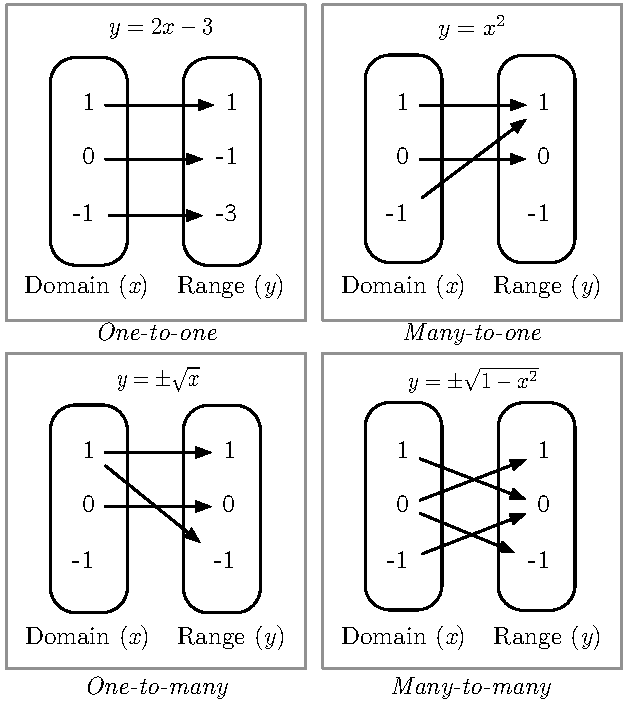
\includegraphics{figures/types_of_mapping}}
\caption{The four mapping classes}
\label{fig:types_of_mapping}
\end{figure}

	\subsubsection{Mapping as association}

In computer science, a mapping is less commonly referred to as a function and more usually called an \emph{associative array} or a \emph{dictionary}, though the word \emph{map} is also used \cite{data_structures}. This type of data structure\footnote{What computer scientist call particular ways of storing and organizing data.} is generally the most flexible way for computers store information. An associative array consists of key/value pairs, where the \emph{value} is the data to be stored and the \emph{key} is the reference to that data. 

\begin{table}
\centering
\Tcaption{An example of key/value pairs (contries and currencies)}
\label{tab:key_value_pairs}
\begin{tabular}{l l}
\hline\hline
key&value\\
\hline
Canada&Dollar\\
France&Euro\\
Bahrain&Dinar\\
Germany&Euro\\
Angola&Kwanza\\
USA&Dollar\\
\hline
\end{tabular}
\end{table}

In table \ref{tab:key_value_pairs} the data is non-numeric and associations between keys and values are arbitrary (from a mathematical point of view). There obviously exists no distinct function that can transform a countries name into the name of its currency, thus the computer must explicitly remember the associations between the words in the form of a \emph{hash table}. At the lowest level, computers store information on a vast array of zeros and ones, and the value ``Kwanza'' only arises through a non-trivial process of encoding and decoding. In order to retrieve it the computer \emph{must} know where it can be found. The hash table takes the input of a key, finds the address for the value and returns it. In this way the hash table is literally the association between two sets of data and thus the mapping between them. 

The four mapping classes outlined in the above section are not limited to the functional domain. The associative array in table \ref{tab:key_value_pairs} is another example of a many-to-one mapping, as many countries have the same currency name. In this vain a one-to-many mapping could be the same keys with values switched to ``Former Monarchs'' (``France'' would map to both ``Louis XVI'' and ``Napoleon III'', etc), while a value of ``Official Languages'' would be a many-to-many mapping (``Canada'' maps to both ``English'' and ``French'' while both ``Canada'' and ``France'' map to ``French'').

Though most applicably represented in computer science, data structures like associative arrays appear in many other fields. Library card catalogs (one-to-one), multilingual dictionaries (many-to-many) and address books (many-to-one) are all very straightforward instances of key/value pairs. In a library card catalog the call number even acts as a sort of hash table. In a large library, a book that is placed in the incorrect position on the shelves will likely be lost for a very long time. Thus the system must remember the keys (titles) and associated values (the books themselves) but also their positions in memory, their call numbers.

The above concepts from mathematics and computer science supply a base of knowledge for understanding mappings theoretically and provide a starting point for analyzing them in a musical context.

%%%%%%%%%%%%%%%%%%%%%%%%%%%%%%%%%%%%%%%%%%%%%%%%%%%%%%%%%%%%%%%%%%%%%%%%%%%%%%%%%%%%%%%%%%%%%%%%%%%%%%%%%%%%%%%%%%%%%%%%%%%%%%%%%%%%%%%%%%%%%%%%%%
\subsection{Mapping for Digital Musical Instruments} \label{sec:mappingforDMIs}

With an acoustical musical instrument a musician must interact directly with the physical object that produces the sound. In this context, the concepts of ``control surface,'' and ``synthesis devices'' are not very relevant, as they are intrinsically linked. With an acoustic guitar the pick \emph{could} be considered to be a sort of control device (as it is primarily used for instrumental interaction), with the strings and body a acting as the sound producing section. The problem with this type of approach is that changing the material of the pick, perhaps to give a different feel for the player, will also necessarily modify the sound produced. The same can be said for modifying nearly any aspect of an acoustic instrument: it will change both the control interface and the created sound. This coupling of parameters causes any concept of a \emph{mapping layer} to be irrelevant.

As stated in the introduction, this is not the case for electronic instruments \shortcite{wanderley}. Electronic sensors transduce musical gestures into signals, which are in turn converted into auditory phenomena by amplifiers and speakers. Any arbitrary transformation can happen to the signals\footnote{Especially digital signals, which are remarkable for their robustness and mutability.} in between these two phases. This flexibility is most obvious with outlandish novel instruments like (TODO: maybe pictures?), but is fundamentally true for any electronic instrument. An electric guitar senses gesture with a magnetic pickup that transforms the signal of a vibrating string into an electronic signal, which is made audible by an amplifier. Though this can happen directly, more or less reproducing the sound of an acoustic guitar, it is also possible to greatly modify this signal before it is amplified, creating tones that may be unrecognizable as the original acoustic instrument.

	\subsubsection{The Mapping Layer}

In response to the importance of this uncoupling of parameters, electronic instruments are often conceptualized as having three independent layers \cite{gestural_control_sound_synthesis}: (TODO diagram)

	\begin{itemize}
		\item The ``gestural controller'': The device with which the musician interacts directly. It generally has sensors that collect gestural data and can provide haptic feedback. The generated signals are output into the mapping layer.
		\item The ``sound generation unit'': This device receives input signals from the mapping layer and uses them to generate sound. This layer can contain melody generating algorithms, sound modifying effects, physical models of acoustical instruments or any other construct that is directly used to produce sound.
		\item The ``mapping layer'': The abstract space that receives input signals from the gestural controller that are output to the sound generation unit. These signals can be connected and modified independently of actions in the other two layers.
	\end{itemize}

As can be seen above, the words ``output'' and ``input'' become ambiguous, whether one is talking from the perspective of the devices (control devices \emph{output} signals that are \emph{input} into the synthesis devices) or the perspective of the mapping layer (the mapping receives \emph{input} from the controller which is \emph{output} to the synthesizer). For the detailed analysis of mappings and mapping devices, this can obviously create confusion \cite{vizmapper}. To avoid this, signals arriving at the mapping layer from the control surfaces will be referred to as \emph{source signals} and signals sent from the mapping layer to the sound generation units will be called \emph{destination signals} for the remainder of this thesis. This follows the nomenclature described in \shortciteN{new_libmapper} and the libmapper API in general.

	\subsubsection{Functional Versus Systems Perspective on Mapping}

Both the more mathematical perspective of mapping as functions and the computer science standpoint of mapping as association are relevant to DMI design. These two concepts are often referred to as the \emph{functional} and the \emph{systems} points of view for mapping, respectively \cite{two_types_of_mapping}. 

Once two signals are connected, say the position of a knob and the cutoff frequency of a low-pass filter,\footnote{A standard synthesis parameter that controls the brightness of a sound, think of the difference between the vowel `o' in `food' (low cutoff) and the vowel `a' in `sad' (high cutoff).} it is very possible that the raw numbers sent from the knob are not appropriate as input for the filter. It may be that the knob transmits numbers ranging from 0 - 127 ($2^7$) and the filter accepts numbers from 0 - 1023 ($2^{10}$). As a result the filter will always be more or less closed no matter how the user turns the knob. To account for this, the mapping needs to \emph{scale} the source signal (by a factor of 8) to fit the destination range. This is a functional kind of mapping, analogous to section \ref{sec:mapping_classes}. The source signal may need to be transformed in many ways. 

The other, higher-level perspective on mapping deals with the actual connection of source to destination signals. On any mapping network there can exist several devices, each with numerous signals. The act of associating devices with devices, signals with signals can drastically change the character of a DMI or group of DMIs. This is known as the systems perspective on mapping. It is necessary for libmapper and the GUI to be able to assist with both kinds of mappings.

	\subsubsection{Mapping Strategies}

For expressive musical networks, simple one-to-one mappings are often insufficient.  \citeN{describing_mappings} argues that it is extremely rare to find such associations in acoustic instruments, as the control parameters are usually tightly coupled with several acoustic dimensions. Interfaces with hundreds of knobs and sliders, each one connected to a single sound parameter have thus been found to ``...hinder rather than help expressive musical behavior.'' \citeA{describing_mappings} In practical experiments where mappings of varying complexity are compared, the most complex were generaly found to be the most expressive and useful \cite{mapping_complexity_experiments}. However, \citeN{interpolated_mappings} states that mappings need to be simple enough for the performer to comprehend them. \citeANP{interpolated_mappings} argues for ``...static mappings over dynamic, and simple over complex'' and proposes an algorithmic solution to compute them. These ``interpolated mappings'' are generated by associating single points in the source and destination spaces (i.e. certain performer gestures with certain sounds) and mathematically filling in the spaces between.

One proposed solution to the cognitive complexity of associating many source and destination signals is to create a second mapping layer \shortcite{wanderley}. Instead of dealing with raw sensor output, like acceleration and inclination, musicians can interact with more interesting gestural information such as ``jab'' or ``left-arm swing.'' These ``cooked'' parameters are argued to be more meaningful and useful musical information than the raw signals. This approach is explored in \citeN{mapping_layers} for mapping both to audio and visual synthesis. The conventional wisdom that mappings need to be complex, yet transparent and meaningful all point to the necessity of a tool for the intuitive and expressive configuration of mappings.

%%%%%%%%%%%%%%%%%%%%%%%%%%%%%%%%%%%%%%%%%%%%%%%%%%%%%%%%%%%%%%%%%%%%%%%%%%%%%%%%%%%%%%%%%%%%%%%%%%%%%%%%%%%%%%%%%%%%%%%%%%%%%%%%%%%%%%%%%%%%%%%%%%
\subsection{libmapper}

The McGill Digital Orchestra project\footnote{The McGill Digital Orchestra. [Online]. Available: \url{http://www.music.mcgill.ca/musictech/DigitalOrchestra/}. Accessed July 9, 2013} began in 2006 with the aim of helping researchers  and performers in music technology to work collaboratively in creating hardware and software solutions for live performance with digital technology. The libmapper project began in response to the difficulty of creating dynamic musical mappings in a collaborative setting \shortcite{malloch}. In its most basic state, libmapper is a library for connecting things. As described by its website: 

\begin{quote} 
``libmapper is an open-source, cross-platform software library for declaring data signals on a shared network and enabling arbitrary connections to be made between them. libmapper creates a distributed mapping system/network, with no central points of failure, the potential for tight collaboration and easy parallelization of media synthesis. The main focus of libmapper development is to provide tools for creating and using systems for interactive control of media synthesis.''\footnote{libmapper: a library for connecting things. [Online]. Available: \url{libmapper.org}. Accessed June, 2013}
\end{quote}

Without libmapper, DMI designers are usually required to ``hard-code'' mappings into their designs. This has the disadvantage of being slow to modify, as it might be necessary to re-compile\footnote{A process in which human-readable code is translated into something the computer can understand. This can take anywhere from a few seconds to days.} code any time a change is made. If the DMI is built in a development environment like Max/MSP modifications can be more quickly implemented. Max/MSP is a ``high-level'' abstraction on top of machine readable code, so Max/MSP programs are prone to slowness and cross-compatibility issues, inhibiting collaboration \shortcite{jamoma}. In either implementation it is difficult for someone other than the original designer to modify mappings.

As a low-level library, libmapper does not introduce many abstractions on top of the data and can work quickly. Any device that embeds libmapper in its code can communicate with other devices that have done the same. In a libmapper network devices communicate with one another directly, as opposed to through some centralized network device. This means that less data overall needs to be sent over the network, and failure of a single device (like the router) will not crash the entire system \shortcite{new_libmapper}, an especially dire situation during live performance.

Another advantage of libmapper, which is especially relevant to this project, is the ability to create an administrative device. These ``monitors'' can query libmapper devices for data, and thus collect data on the network overall. Monitors also are able to create, destroy and modify connections on the network. This allows for external visualization and control of a libmapper network.

	\subsubsection{Open Sound Control and libmapper Syntax}

Like any communication, communication between digital devices functions well only when the devices speak the same language. In the Internet age this becomes particularly relevant: the vast array of continuously connected devices, sending and requesting information would instantly collapse if every developer coded to his or her own idiosyncrasies. To prevent this, computer scientists make use of various communication ``protocols'' when creating software. Hypertext Transfer Protocol (HTTP) is the most famous example of such a system.

At its core, libmapper builds its on language on top of the Open Sound Control (OSC) protocol, as described by \shortciteN{osc}. OSC defines the format for messages that are sent between sound producing devices (as implied by the name), but can also be used for related multimedia devices such as stage lights or vibrating motors. It provides means for flexible, high-resolution communication and was intended to replace MIDI\footnote{MIDI Manufacturers Association - The official source of information about MIDI. [Online]. Available: \url{www.midi.org}. Accessed July 11, 2013}, the 30-year-old standard for musical instrument communication. 

OSC formats messages much like Internet URLs, arbitrary strings of characters separated by `/' characters. libmapper messages also take on this format, using the structure to expose hierarchy of signals:

	\begin{itemize}
	\item\url{tstick.1/raw/accelerometer/1/x}: The data for the `x' dimension of the first accelerometer of the first instrument of class ``tstick'' on the network (see TODO for a description of the gestural controller T-Stick). Here the word ``raw'' denotes that no pre-processing has been applied to this signal. 
	\item\url{tstick.1/raw/accelerometer/2/y}: A signal transmitting the data for the same instrument as above, but the `y' dimension of the second accelerometer.
	\item\url{tstick.1/cooked/accelerometer/2/amplitude}: A ``cooked'' signal. All three dimensions of accelerometer 2 are combined to compute the overall acceleration of the point. These signals can also be cooked to expose angle and elevation as signals.
	\item\url{granul8.2/filter/evelope/frequency/low}: The data for the low-end cutoff for the shape of the filter for the instrument named ``granul8.2'' (a granular synthesizer, thus a destination device).
	\end{itemize}

This structure of signal names aims to be semantically relevant, and allows a GUI to display hierarchical structure of networks. Any one of the above signals transmits not only the signal's value, but also metadata. Signal metadata usually includes data type, length (single number vs. vector), units like volts or meters per second, maximum value and minimum value. Designers can ``tag'' signals with any extra metadata they may wish to add, such as physical position, color or owner's name. In the GUI it is necessary to allow users to view and manipulate any arbitrary kind of signal metadata.

To make signal names as coherent and consistent as possible, libmapper makes use of the \emph{Gesture Description Interchange Format} (GDIF) \shortcite{GDIF}, which provides a standard for motion capture data. Structures are given short, semantically relevant names. GDIF also provides a standard vocabulary for describing motion with dimensions such as ``weight,'' ``space,'' ``time'' and ``flow.'' 

	\subsubsection{Structure of libmapper Networks}

Data organized into a time series. Conceptually a signal is continuous, however our use of the term signal will refer to discretized signals, without assumptions regarding sampling intervals.
signals, devices, expressions
In order to maintain internal consistency, libmapper introduces a naming convention of its own. A libmapper \emph{device} 

\begin{figure}[ht]
\centering
	\scalebox{1}{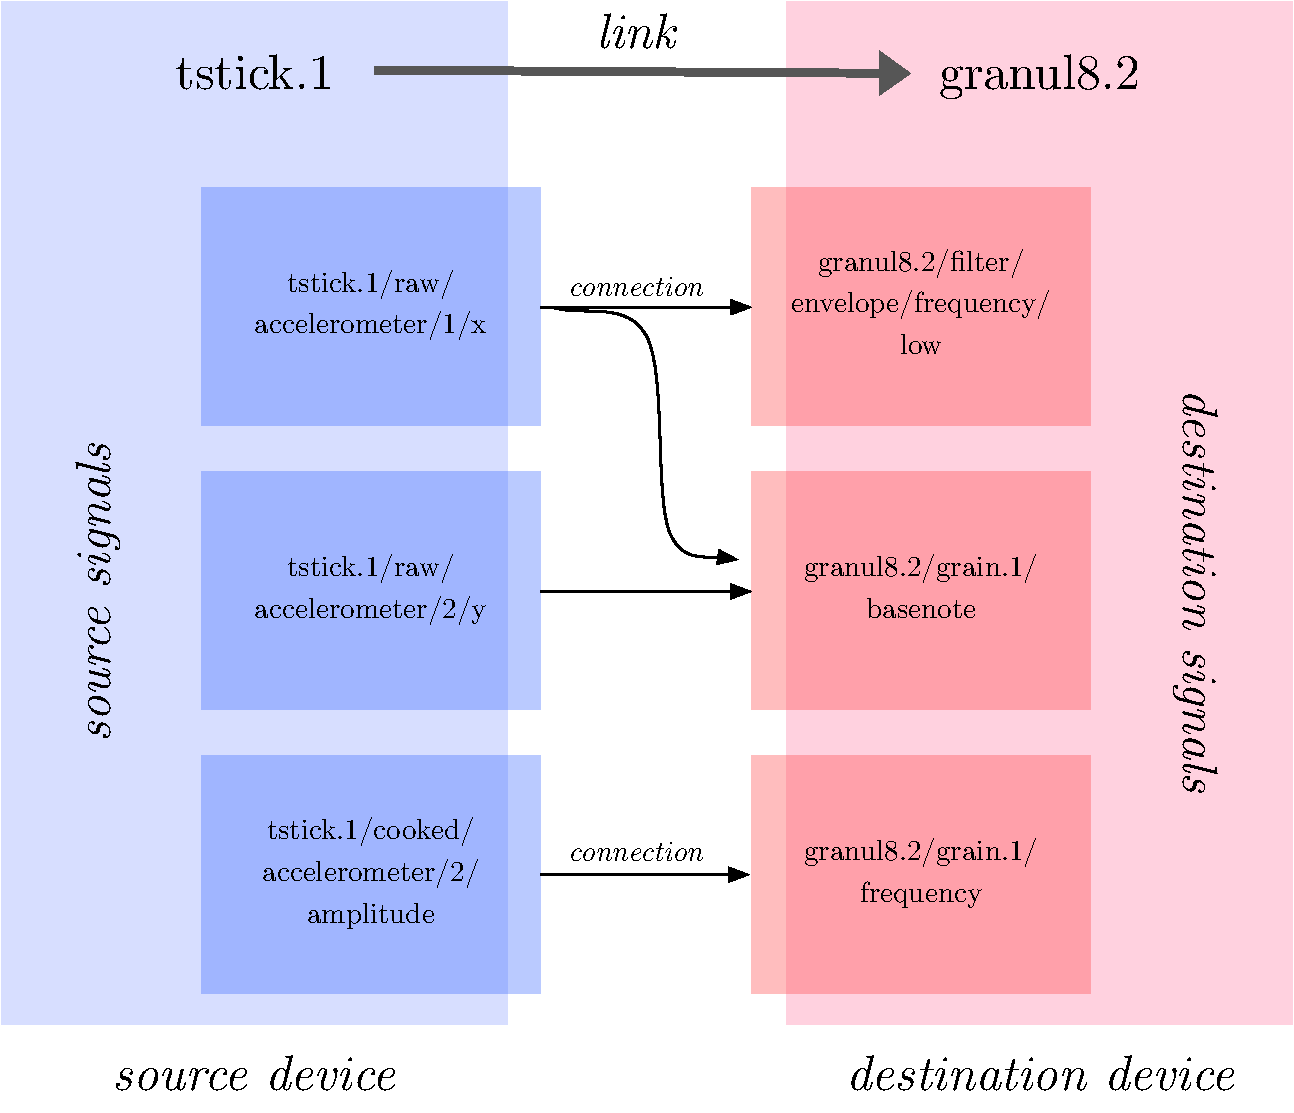
\includegraphics{figures/libmapper_devices}}
\caption{A simple libmapper network}
\label{fig:libmapper_devices}
\end{figure}

	\subsubsection{Control of libmapper Devices and Signals}
expression, range (source and dest), signal mode (linear, calibrate, bypass, expression), mute, send as instance?

%%%%%%%%%%%%%%%%%%%%%%%%%%%%%%%%%%%%%%%%%%%%%%%%%%%%%%%%%%%%%%%%%%%%%%%%%%%%%%%%%%%%%%%%%%%%%%%%%%%%%%%%%%%%%%%%%%%%%%%%%%%%%%%%%%%%%%%%%%%%%%%%%%
%%%%%%%%%%%%%%%%%%%%%%%%%%%%%%%%%%%%%%%%%%%%%%%%%%%%%%%%%%%%%%%%%%%%%%%%%%%%%%%%%%%%%%%%%%%%%%%%%%%%%%%%%%%%%%%%%%%%%%%%%%%%%%%%%%%%%%%%%%%%%%%%%%
\section{Data Visualization}


The graphical user interface described in this thesis presents users with solely visual information. As it is a tool to be used with primarily sound producing objects auditory feedback is problematic and common digital devices (laptops, tablets, etc.) provide us with no means of producing haptic response. Mapping systems can contain tremendous amounts of information: device names, digital addresses, numbers of signals, signal names, units, ranges, data types, expressions, parent devices and any kind of meta-data a libmapper user may choose to add to his or her devices. As a result, it is necessary a review how best to visually represent vast amounts of structured data.

\subsection{Graphical Perception}
	\subsubsection{Heirarchical Structures}
	\subsubsection{Dense Information}
\subsection{Visualization Techniques}
	\subsubsection{Filtering}
	\subsubsection{Spark Lines}
	\subsubsection{Dash Plots}
\subsection{Visualization Systems}
	Allosphere?, Braun Braun: view OSC data flows \shortcite{braun}, HEB?
\begin{enumerate}
	\item Allosphere? :\shortcite{allosphere}
	\item Heirarchical edge bundling: \shortcite{HEB}
	\item Tukey: \shortcite{tuckey}
	\item Envisioning information: \shortcite{tufte1}
	\item Beautiful Evidence: \shortcite{tufte2}
	\item The other Tufte book I have at home.
	\item OSC data flows with Braun \shortcite{braun}
\end{enumerate}

%%%%%%%%%%%%%%%%%%%%%%%%%%%%%%%%%%%%%%%%%%%%%%%%%%%%%%%%%%%%%%%%%%%%%%%%%%%%%%%%%%%%%%%%%%%%%%%%%%%%%%%%%%%%%%%%%%%%%%%%%%%%%%%%%%%%%%%%%%%%%%%%%%
%%%%%%%%%%%%%%%%%%%%%%%%%%%%%%%%%%%%%%%%%%%%%%%%%%%%%%%%%%%%%%%%%%%%%%%%%%%%%%%%%%%%%%%%%%%%%%%%%%%%%%%%%%%%%%%%%%%%%%%%%%%%%%%%%%%%%%%%%%%%%%%%%%
\section{User Interface Design}

\subsection{A Brief History of Electronic User Interfaces}
\subsection{Task Analysis}
\subsection{Recall and Recognition?}
\subsection{Collaborative Network Interfaces}
	MPG Care Package \shortcite{MPGcarepackage}
\subsection{The Model-View-Controller Architecture}
	MVC Krasner Pope \shortcite{MVC_krasnerpope}
\subsection{User Centric Design}
	Organizational context \shortcite{usd}
	Usability testing \shortcite{usd_corry}
	Information professionals \shortcite{usd_schulze}
\begin{enumerate}
	\item Inclusive interconnections \shortcite{inclusiveinterconnections}
	\item Sense Stage \shortcite{senseStage}
\end{enumerate}

%%%%%%%%%%%%%%%%%%%%%%%%%%%%%%%%%%%%%%%%%%%%%%%%%%%%%%%%%%%%%%%%%%%%%%%%%%%%%%%%%%%%%%%%%%%%%%%%%%%%%%%%%%%%%%%%%%%%%%%%%%%%%%%%%%%%%%%%%%%%%%%%%%
%%%%%%%%%%%%%%%%%%%%%%%%%%%%%%%%%%%%%%%%%%%%%%%%%%%%%%%%%%%%%%%%%%%%%%%%%%%%%%%%%%%%%%%%%%%%%%%%%%%%%%%%%%%%%%%%%%%%%%%%%%%%%%%%%%%%%%%%%%%%%%%%%%
\section{Relevant User Interfaces}

\subsection{Junxion}
	Junxion \shortcite{junxion}
\subsection{Osculator}
	Osculator: mapping OSC stuff \shortcite{osculator}
\subsection{Other Similar Interfaces}
	mpgcarepackage?
	Integra \shortcite{integra}
	Eaganmatrix: GRID VIEW! \shortcite{eaganmatrix}
	Patchage: a linking, dragging, connecting interface \shortcite{patchage}
\subsection{Prior Interfaces for libmapper} \label{sec:priorGUIs}
	Vizmapper \shortcite{vizmapper}


%%%%%%%%%%%%%%%%%%%%%%%%%%%%%%%%%%%%%%%%%%%%%%%%%%%%%%%%%%%%%%%%%%%%%%%%%%%%%%%%%%%%%%%%%%%%%%%%%%%%%%%%%%%%%%%%%%%%%%%%%%%%%%%%%%%%%%%%%%%%%%%%%%
%%%%%%%%%%%%%%%%%%%%%%%%%%%%%%%%%%%%%%%%%%%%%%%%%%%%%%%%%%%%%%%%%%%%%%%%%%%%%%%%%%%%%%%%%%%%%%%%%%%%%%%%%%%%%%%%%%%%%%%%%%%%%%%%%%%%%%%%%%%%%%%%%%
\section{Summary}
	
%
\typeout{}
%!TEX root = ../thesis.tex
\chapter{Design \& Implementation}

	Development of a graphical user interface for libmapper creates a unique challenge. Obviously such an interface is a practical tool, and should function as such, yet it also must work in concert with DMIs which are inherently designed for creative use. For the purposes of this project, the assumed solution to this innate paradox is to provide the user with multiple independent modes of control.  libmapper itself is an extremely flexible API that makes few assumptions as to the network of devices and signals or how they are mapped. It is thus fitting that a GUI for libmapper would be equally as flexible. In lieu of a single perfect solution for network visualization and interactivity, providing users with various independent solutions provided a good compromise.

	Work began with the webmapper interface described in section \ref{sub:webmapper}. An MVC structure was built around the code in order to make the program more extensible and allow for the easy integration of multiple views. Missing features from Maxmapper are incorporated into the main view mode, known as the ``list'' view. That interface has been extended in various ways, taking advantage of the new code base. Two new view modes, the ``grid'' and ``hive'', both designed by Jonathan Wilansky at IDMIL, are integrated into the main GUI. Finally, the code has been compiled together as a standalone application, ready for wide distribution.

%%%%%%%%%%%%%%%%%%%%%%%%%%%%%%%%%%%%%%%%%%%%%%%%%%%%%%%%%%%%%%%%%%%%%%%%%%%%%%%%%%%%%%%%%%%%%%%%%%%%%%%%%%%%%%%%%%%%%%%%%%%%%%%%%%%%%%%%%%%%%%%%%%%%%%%%%%%%%%%%%%%%%%%%%%%%%%%%%%%%%%%%%%%%%%%%%%%%%%%%%%%%%%%%%%%%%%%%%%%%%%%%%%%%%%%%%%%%%%%%%%%%%%%%%%%%%%%%%%
\section{Development of a Flexible System} % (fold)
\label{sec:development_of_a_flexible_system}

Prior GUIs for libmapper have been successfully used for some time, but all have failed to become a standard for the same reason: they cannot accommodate all possible use-cases of libmapper. List based views like the Max/MSP GUI and webmapper cannot show hierarchies while the cluster view implemented in vizmapper can be overly cumbersome for interaction with simple networks. Especially with so much work already completed on prior GUIs, it is more suitable to integrate different approaches into a single GUI than to begin work on some new, hopefully superior approach that would likely prove to be flawed like all that came before it. 

Interface integration is accomplished through an extremely simple approach: a drop-down menu is added to the upper left corner of the interface. Options on this menu represent different visualization modes available to the user. By selecting a new visualization mode the GUI drastically changes it appearance, replacing nearly every visual element in the display.
	%Needs to be adaptable, show any metadata

	\subsection{MVC architecture} % (fold)
	\label{sec:mvc_architecture}

Because a modular design is desired, the Model-View-Controller (MVC) metaphor for structuring software applications \cite{MVC_krasnerpope} is used as a general framework for structuring the application. In fact, the whole scale swapping in and out of independent visual modes would be straightforward implementation of MVC. Unfortunately, the \url{libmapper} $\rightarrow$ \url{python monitor} $\rightarrow$ \url{browser} implementation is slightly more complicated than as imagined by \citeANP{MVC_krasnerpope}. Figure \ref{fig:mapper_network} can be contrasted with (TODO). A few layers of abstraction are added to take into account the monitor, the network itself and control features independent to the view (see section \ref{sec:top_toolbar}), but the general MVC architecture is maintained.

\begin{figure}[!ht]
\centering
	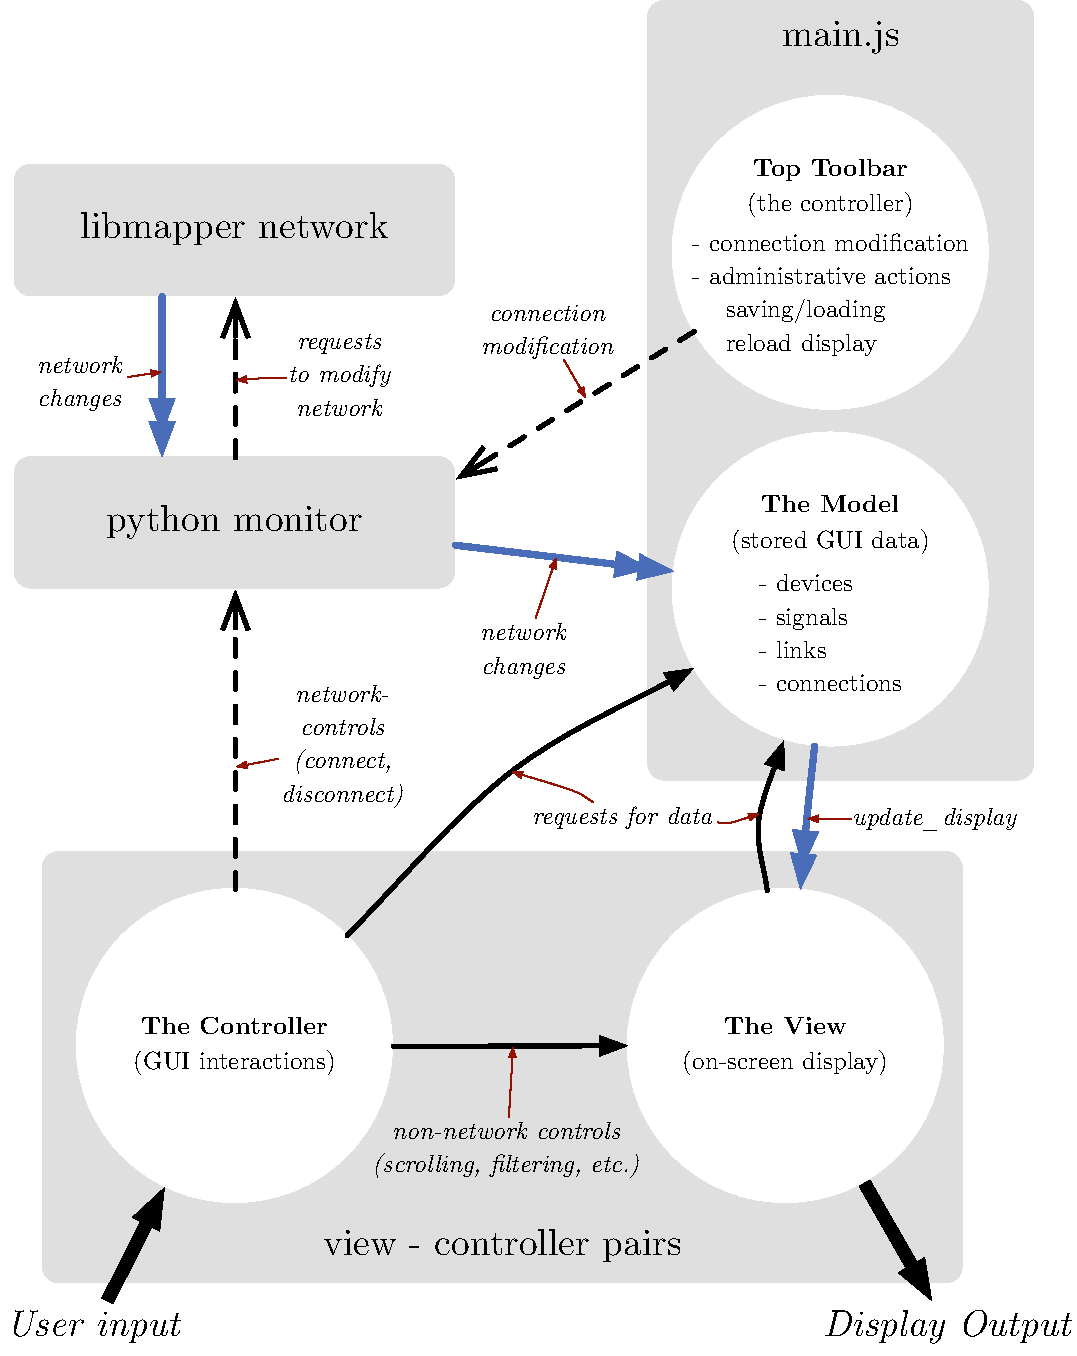
\includegraphics[width=0.8\textwidth]{figures/mapper_network}
\caption{MVC hierarchy for the GUI and libmapper, blue arrows show propogation of network changes, dashed arrows denote messages requesting a network change.}
\label{fig:mapper_network}
\end{figure}


		\subsubsection{Independent communication}

First and foremost, it is essential that data on the screen should reflect data on the network. This is not entirely straightforward, as asynchronous messages are constantly being sent from the GUI to libmapper and vice versa. In a truly distributed system, data on the libmapper network will be constantly changing as other users add devices and modify mappings. As can be seen in figure \ref{fig:mapper_network}, the actual libmapper network, the displayed data and user interaction are very insulated from one another. For example, a user command to link two devices (in this case \url{source.1} and \url{dest.1}), the following message will be sent to the python monitors:

\url{ {"cmd":"link","args":["/source.1","/dest.1"]} }

Meaning: a linking command is sent to \url{source.1} and \url{dest.1} (the command itself is a python dictionary). After this, the display will not do anything, as the display has not yet been notified of the link. The monitor then relays this message to the network, using libmapper specific syntax. If the link is successful, the monitor receives notice, and sends a message to the main javascript file:

\url{("new_link", {"src_name": "/source.1", "dest_name": "/dest.1"}) }

This states that a new link has been formed between the source device \url{source.1} and the destination device \url{dest.1}. Only then does the GUI respond to the change on the network. Signal data itself is not available to the GUI in any way, as libmapper networks are designed to prevent this kind of bandwidth clutter \shortcite{new_libmapper}.

		\subsubsection{The model}

The model consists of an abstract copy of the network, residing on the local machine. Independent views can consult these data, but cannot directly modify it. Messages from the python monitor announce new links, modifications to connections, or any other changes on the network. All of these changes are recorded and reflected in the model. The model itself consists of four data structures.

\begin{itemize}
 	\item \textbf{Devices}: Storage of all present devices and device metadata.
 	\item \textbf{Links}: A record of all links presently on the network.
 	\item \textbf{Signals}: Keeps track of signals on the network, but only whichever signals are currently visible in the GUI. This is done to save bandwidth and processing power. View-controller pairs keep track of which devices are currently being viewed, and can ask for their child signals. 
 	\item \textbf{Connections}: All connections and connection metadata between signals currently in the model.
 \end{itemize} 

It is possible that previously viewed signals will persist in the model, but they and their connections will not be updated upon change.

		\subsubsection{View-controller pairs}

All interaction handlers\footnote{Response to mouse clicks and certain keypresses.} and visualizations are stored in modular, view-controller pairs, as recommended by \citeN{MVC_krasnerpope}. Each view controller pair corresponds with a single view mode. Pairs can have any combination of UI handlers and visual features, but must have the following four functions that are called by the main file on which the model is stored:

\begin{itemize}
	\item \url{view.initialize()}: Calls upon the view to create its visual elements and add 
	\item \url{view.get_focused_devices()}: Returns whichever devices are currently visible in the view. This is used for populating the signal and connection data structures.
	\item \url{view.cleanup()}: Causes the controller to remove all interaction handlers.
	\item \url{view.update_display()}: Called whenever the model changes. The view is not aware
\end{itemize}


		%initialize, cleanup, update_display
	
	% subsection mvc_architecture (end)

	\subsection{Top toolbar} % (fold)
	\label{sec:top_toolbar}

Certain tasks and information providing structures are sensible to include across visualization modes. In light of this, a static toolbar is presented at the top of the GUI. This toolbar contains all administrative controls and connection modification fields. 

\begin{figure}[!h]
\centering
	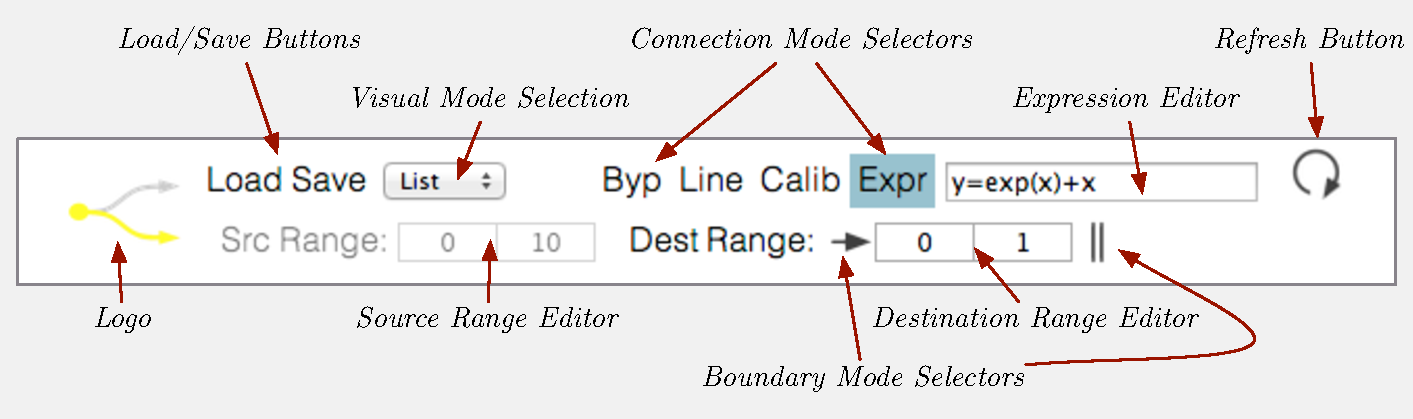
\includegraphics[width=1\textwidth]{figures/top_toolbar}
\caption{The upper toolbar}
\label{fig:toolbar}
\end{figure}

\begin{itemize}
	\item \textbf{Administrative controls}
	\begin{itemize}
		\item\emph{Load/Save buttons}: These elements respond to clicks and save and load mappings, as discussed in section \ref{sec:saving_and_loading}.
		\item\emph{Visual mode selection}: A drop-down menu containing all possible view modes (at the writing of this thesis: List, Grid and Hive).
		\item\emph{Refresh Button}: When clicked, all data residing on the GUI is erased and re-gathered. This is useful if the monitor somehow desynchronizes with the network.
	\end{itemize}

	\item \textbf{Connection modification}
	\begin{itemize}
		\item\emph{Connection mode selectors}: If a single connection is selected within the GUI, this array of buttons allows the user to choose between the available connection modes.
		\item\emph{Expression editor}: Here the user inputs a custom expression, if in ``Expr'' mode, in other modes this field displays the connection's expression but is not editable.
		\item\emph{Source range editor}: These two numbers reflect the maximum and minimum values of the input signal, is only editable in the ``Line'' connection mode.
		\item\emph{Destination range editor}: Same as above but for the destination signal. Due to boundary conditions these fields are useful in all modes.
		\item\emph{Boundary mode selectors}: Two buttons that cycle through five boundary modes for both the maximum and minimum destination value. A graphic exists to represent each mode.
	\end{itemize}
\end{itemize}

All interface features not present in the top toolbar are part of the current visualization mode and are placed into a ``container'' element below, occupying the remainder of the window.

	% subsection top_toolbar (end)



% section development_of_a_flexible_system (end)

%%%%%%%%%%%%%%%%%%%%%%%%%%%%%%%%%%%%%%%%%%%%%%%%%%%%%%%%%%%%%%%%%%%%%%%%%%%%%%%%%%%%%%%%%%%%%%%%%%%%%%%%%%%%%%%%%%%%%%%%%%%%%%%%%%%%%%%%%%%%%%%%%%%%%%%%%%%%%%%%%%%%%%%%%%%%%%%%%%%%%%%%%%%%%%%%%%%%%%%%%%%%%%%%%%%%%%%%%%%%%%%%%%%%%%%%%%%%%%%%%%%%%%%%%%%%%%%%%%
\section{Integration of Interface Features} % (fold)
\label{sec:integration_of_interface_features}

Development began by unifying features of the Maxmapper onto the Webmapper code. Webmapper was selected as a starting point because of cross-platform nature of a web-based implementation. The general two-table structure of Maxmapper and Webmapper created the first view of the interface, known as the ``list'' view.

	\subsection{Structure of the list view} % (fold)
	\label{sub:the_list_view}

The list view provides the most straightforward way to visualize and interact with libmapper. Two tables dominate the visible area, listing source elements on the left and destination elements on the right. B\'ezier curves form lines between associated list elements on each each list. Because these curves do not always represent the same data structures, the lines themselves are referred to as \emph{arrows} by the GUI code, and by this document.

\begin{figure}[ht]
\centering
	\scalebox{0.4}{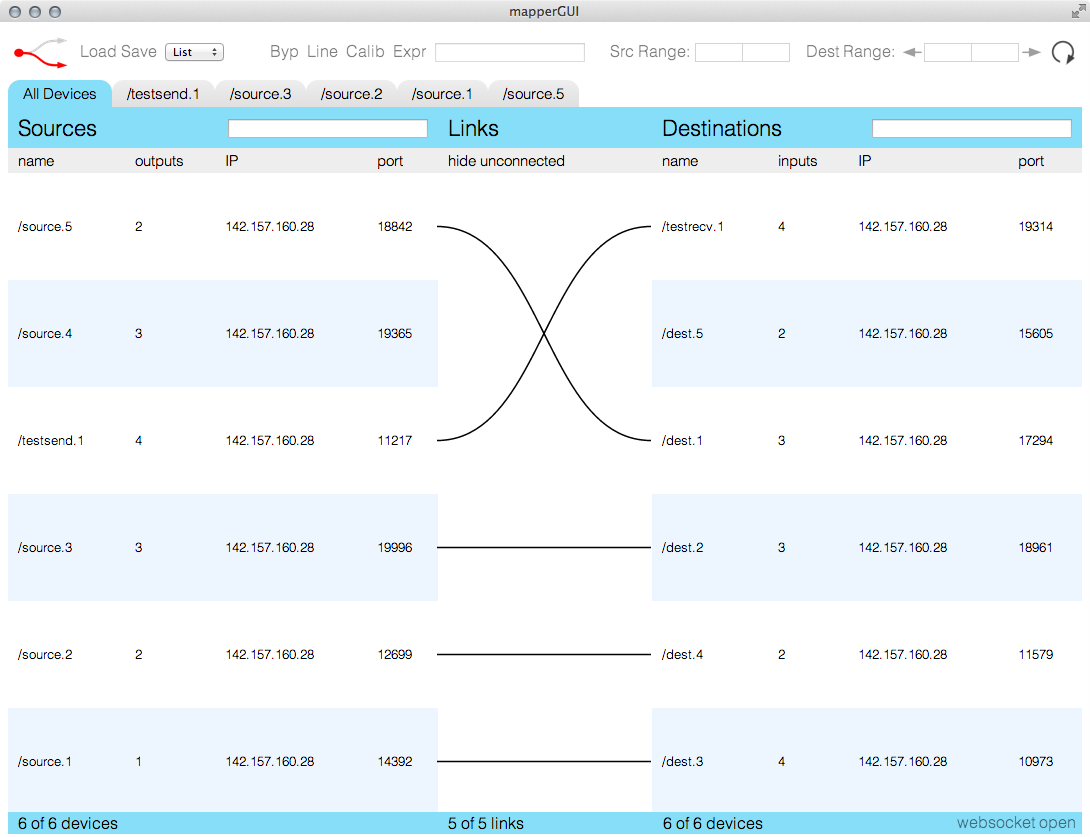
\includegraphics{figures/list_view_all_devices}}
\caption{The list view with all devices selected}
\label{fig:list_view_all_devices}
\end{figure}

The view itself is divided into two major modes: ``All Devices'' and individual linked source devices. Switching between these modes is accomplished through tabs that appear at the top of the container, much like the tabs that appear in modern web browsers. In the All Devices tab, every device displayed on the network is listed in one of the two columns, as in \ref{fig:list_view_all_devices}. Source devices are listed in the left table, while the right table lists destination devices. Intermediate devices, such as implicit mappers described in \cite{interpolated_mappings}, will be listed in both tables. Here arrows represent links between devices. Currently the GUI provides users with names, the number of child signals, IP addresses and a port for every device. Since no connections or signals are displayed, most of the top bar (see section \ref{sec:top_toolbar}) is disabled in the All Devices tab. Saving and loading are also disabled.

\begin{figure}[ht]
\centering
	\scalebox{0.4}{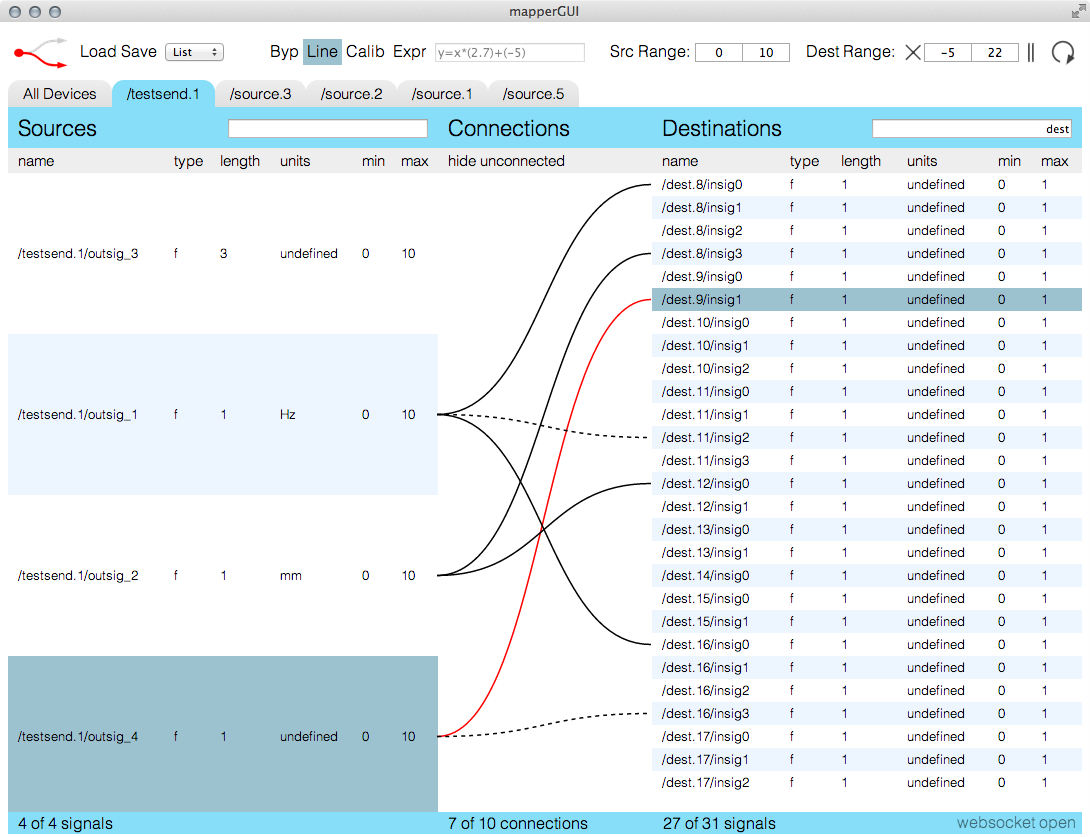
\includegraphics{figures/list_view_single_link}}
\caption{The list view with device \textbf{testsend.1} selected}
\label{fig:list_view_single_link}
\end{figure}

The GUI draws a tab for every source device with at least one link to a destination device. Clicking on any of these devices will redraw both tables. The left table now shows all child signals for the selected source device while the right table displays child signals for every destination device linked to the selected device. 

	% subsection the_list_view (end)
	
	\subsection{Display libmapper metadata} % (fold)
	\label{sub:display_libmapper_metadata}

The original webmapper interface tables listing devices and signals have no headers. Without these queues, only a small amount of metadata is provided (see figure \ref{fig:webmapper}):

\begin{table}
	\centering
	\Tcaption{Metadata available in webmapper vs list view}
	\label{tab:webmapper_list_view_metadata}
		\begin{tabular}{l  l  |  l l }
		\hline\hline
		\textbf{webmapper}&&\textbf{list view}\\
		Devices&Signals&Devices&Signals\\
		\hline
		name&name&name&name\\
		IP address&data type&IP address&data type\\
		port&vector length&port&vector length\\
		&&number of inputs&units\\
		&&number of outputs&maximum value\\
		&&&minimum value\\
		\end{tabular}
\end{table}

To include a necessary feature of max mapper, column headers are added to the list view. Also included are the new pieces of device and signal metadata listed in table \ref{tab:webmapper_list_view_metadata}. Tables draw themselves with invisible extra columns, such that adding extra data can be easily accomplished. If a user embeds extra metadata not listed above onto devices or signals, that data will automatically be included in the table display.  

In general, the GUI tries to keep possible extensions to libmapper like this in mind. Very little is assumed about the network itself. In turn, the only device metadata that \emph{must} exist is the name and number of inputs/outputs, which is used to either display the device as a source or destination. For signals, the GUI takes vector length into account when deciding whether two signals are compatible and can be connected. However, disincluding length in the signal metadata will not result in an error.
	
	% subsection display_libmapper_metadata (end)

	\subsection{Visual feedback} % (fold)
	\label{sub:visual_feedback}
		% # of signals/etc.
		% muted lines
		% row striping

	% subsection visual_feedback (end)

	\subsection{Namespace filtering} % (fold)
	\label{sub:namespace_filtering}
		%hide unconnected signals
	% subsection namespace_filtering (end)

	\subsection{Draggable connections and links} % (fold)
	\label{sub:draggable_connections_and_links}
	
	% subsection draggable_connections_and_links (end)

% section integration_of_interface_features (end)

%%%%%%%%%%%%%%%%%%%%%%%%%%%%%%%%%%%%%%%%%%%%%%%%%%%%%%%%%%%%%%%%%%%%%%%%%%%%%%%%%%%%%%%%%%%%%%%%%%%%%%%%%%%%%%%%%%%%%%%%%%%%%%%%%%%%%%%%%%%%%%%%%%%%%%%%%%%%%%%%%%%%%%%%%%%%%%%%%%%%%%%%%%%%%%%%%%%%%%%%%%%%%%%%%%%%%%%%%%%%%%%%%%%%%%%%%%%%%%%%%%%%%%%%%%%%%%%%%%
\section{Extension of Control and Visual Elements} % (fold)
\label{sec:extension_of_control_and_visual_elements}

	\subsection{Keyboard shortcuts} % (fold)
	\label{sec:keyboard_shortcuts}

		%select all, large selections
	
	% subsection keyboard_shortcuts (end)

	\subsection{Window resizing} % (fold)
	\label{sec:window_resizing}
	
	% subsection window_resizing (end)

	\subsection{Variable line heights} % (fold)
	\label{sec:variable_line_heights}
	
	% subsection variable_line_heights (end)

	\subsection{Visual Redesign} % (fold)
	\label{sec:visual_redesign}
	
	% subsection visual_redesign (end)

	\subsection{Grid \& Hive views} % (fold)
	\label{sec:grid_&_hive_views}

\begin{figure}[ht]
\centering
	\scalebox{0.4}{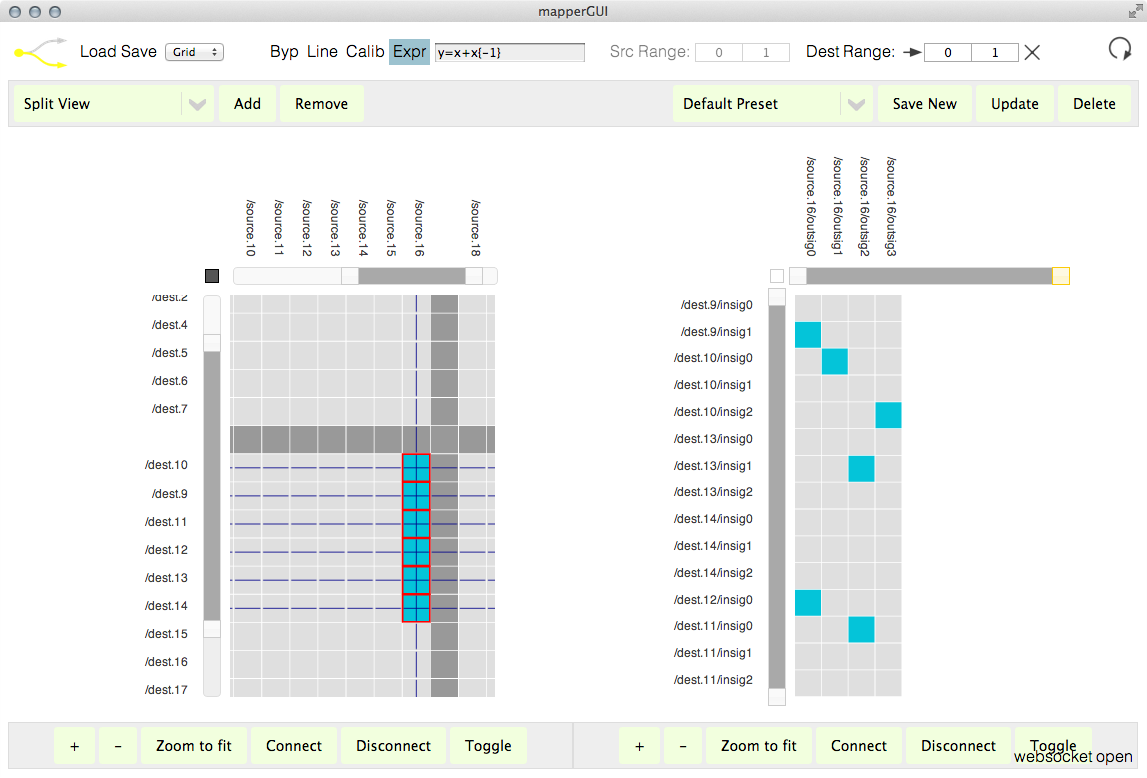
\includegraphics{figures/grid}}
\caption{The grid view}
\label{fig:grid}
\end{figure}

\begin{figure}[ht]
\centering
	\scalebox{0.4}{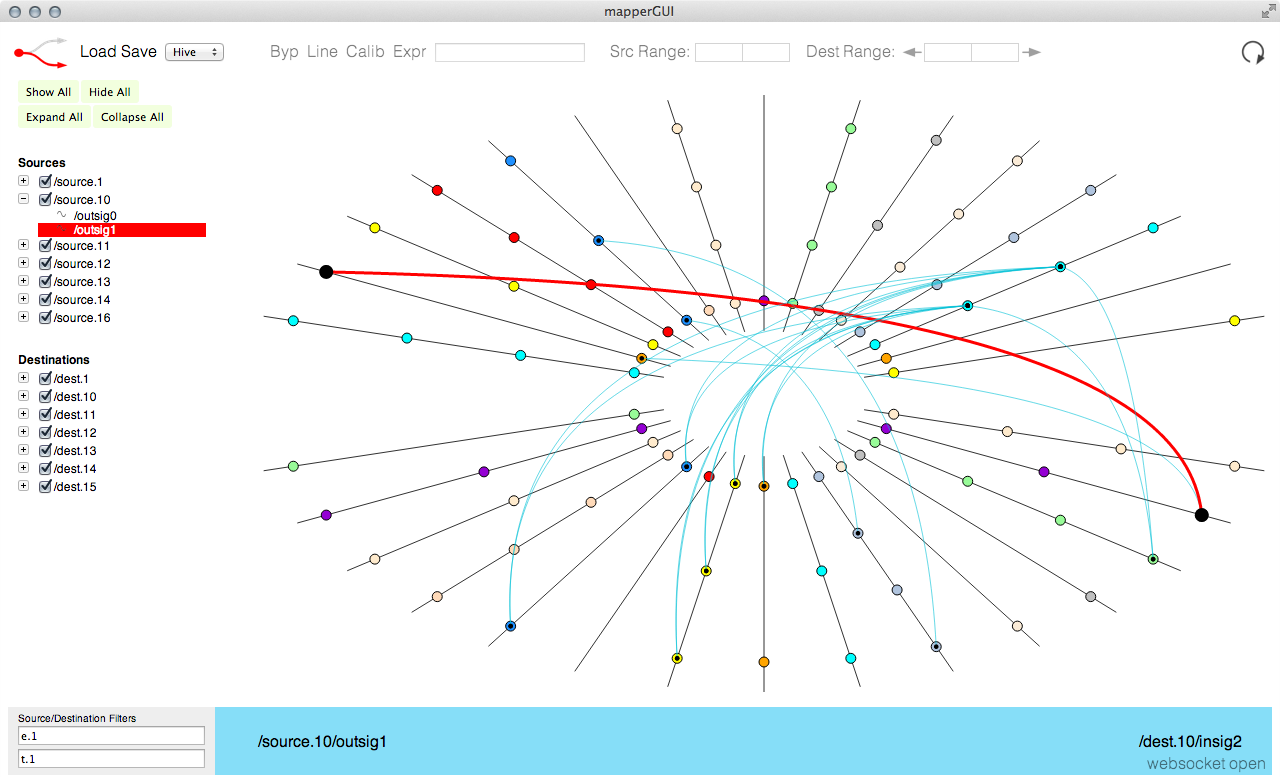
\includegraphics{figures/hive}}
\caption{The hive view}
\label{fig:hive}
\end{figure}
	
	% subsection grid_&_hive_views (end)

% section extension_of_control_and_visual_elements (end)

%%%%%%%%%%%%%%%%%%%%%%%%%%%%%%%%%%%%%%%%%%%%%%%%%%%%%%%%%%%%%%%%%%%%%%%%%%%%%%%%%%%%%%%%%%%%%%%%%%%%%%%%%%%%%%%%%%%%%%%%%%%%%%%%%%%%%%%%%%%%%%%%%%%%%%%%%%%%%%%%%%%%%%%%%%%%%%%%%%%%%%%%%%%%%%%%%%%%%%%%%%%%%%%%%%%%%%%%%%%%%%%%%%%%%%%%%%%%%%%%%%%%%%%%%%%%%%%%%%
\section{Other GUI features} % (fold)
\label{sec:other_gui_features}

	\subsection{Saving \& Loading} % (fold)
	\label{sec:saving_and_loading}
	
	% subsection saving_&_loading (end)

	\subsection{Creation of a standalone \& distribution} % (fold)
	\label{sec:creation_of_a_standalone_and_distribution}
	
	% subsection creation_of_a_standalone_&_distribution (end)

% section other_gui_features (end)





%
\typeout{}
%!TEX root = ../thesis.tex
\chapter{Applications \& Discussion}

This chapter presents a discussion of MapperGUI's software design and its consequences for musical mapping, as well as revisions made to the code since initial release. The interface's features are explored in an attempt to evaluate the successes and failures of the design. Feedback from users was gathered throughout the project and through informal interviews after the software's release. This feedback is summarized and presented here. A modification to the code, motivated by feedback from users, is also described. MapperGUI is then compared to similar interfaces, analyzing especially for new features that could be incorporated into our flexible framework. Finally, the system is evaluated overall with respect to the project's initial goals.


%%%%%%%%%%%%%%%%%%%%%%%%%%%%%%%%%%%%%%%%%%%%%%%%%%%%%%%%%%%%%%%%%%%%%%%%%%%%%%%%%%%%%%%%%%%%%%%%%%%%%%%%%%%%%%%%%%%%%%%%%%%%%%%%%%%%%%%%%%%%%%%%%%%%%%%%%%%%%%%%%%%%%%%%%%%%%%%%%%%%%%%%%%%%%%%%%%%%%%%%%%%%%%%%%%%%%%%%%%%%%%%%%%%%%%%%%%%%%%%%%%%%%%%%%%%%%%%%%%
\section{User Feedback} % (fold)
\label{sec:user_feedback}

The entire MapperGUI project began with user feedback from prior GUIs for libmapper. Throughout the design process, functional versions of MapperGUI were provided to libmapper users. Their feedback was crucially important to the evolution of the software. After the first official release of MapperGUI, long-term users were informally interviewed. These users were questioned specifically as to their specific applications of MapperGUI.

Even at this early stage of release, users have already incorporated MapperGUI into a wide variety of projects. This reflects our initial assumptions that a successful GUI must be flexible. Throughout development MapperGUI was used as an experimental tool and aid in designing DMIs. The interface was utilized in concert with motion capture systems, vibrotactile feedback and even loaded onto a Raspberry PI\footnote{Raspberry Pi | An ARM GNU/Linux box for \$25. Take a byte! [Online] Available: \url{http://www.raspberrypi.org}. Accessed August 1, 2013}. During this process users encountered problems, had ideas for extensions and used the GUI in ways we could not have anticipated.



%for response to vibrotactile feedback in a motion-capture study. It was also used in a motion capture setting for the design of an interactive audio installation. In the latter situation MapperGUI was required to handle many signals per single device, as each person in the room required 25 three-dimensional markers (75 signals total). A DMI designer has been using MapperGUI to test mappings for her input device with a single sound synthesizer, each containing about 30 signals.

%MapperGUI is being used as a development tool as well. A programmer is attempting to build a software bridge between libmapper and the Arduino\footnote{}. She uses MapperGUI to test the robustness and effectiveness of the software, and has even successfully loaded the GUI onto a raspberryPI\footnote{}

%\begin{table}
%\begin{center}
%\begin{tabular}{l p{5cm} p{5cm}}
	%\hline\hline
	%user&use case&concerns\\
	%\hline
	%Mailis&Intonespacio&saving and loading\\
	%Hakon&Experimenting with vibrotactile feedback and motion capture systems&Switching between various mappings\\
	%Clayton&An interactive space using motion capture&Reliability of network\\
	%Julie&libmapper code for firmata&Speed of function (she's using a rasperry Pi)\\
	%\hline
	%Andrew Stuart&teaches class with libmapper&\\
	%Gestes (Marlon)&Performance, etc.&Hide unconnected\\
%\end{tabular}
%\end{center}	
%\end{table}
%
%Hakon Knutzen, Mailis Rodrigues, Clayton Mamedes, Julie Ren\'e
		%%Mailis, Clayton, Hakon, Julie


	\subsection{General feedback} % (fold)
	\label{sub:general_feedback}

Most of our users had experience with libmapper, and had attempted to compile and use the library from scratch. Many commented on how well MapperGUI lowered the barriers to entry for non-technical users. Users who had never used libmapper before pointed out how much time had been saved in their work flow, versus hard-coding mappings.

The best reviewed feature of MapperGUI was the automatic linear scaling control found in the top bar. Some users previously detected signal minima and maxima by hand, then directly calculated and applied linear scaling functions. With MapperGUI the task is trivially easy: one must simply enter the desired destination range and set the connection to the \emph{Calibrate} mode. Most of the ``magic'' in this feature is the result of the libmapper API, but providing users access through an easy-to-use GUI is also important. One user expressed frustration because she was not aware this feature existed, and instead continued to painstakingly condition her signals in Max/MSP. She was very impressed over how much time was saved by switching this workload to libmapper and MapperGUI.

Use of the other connection modes was rare. Users found the expression input box difficult and opaque. Directly calculating the appropriate mathematical expression was seen as too abstract. This is a sensible problem to have, as difficult text-based input is precisely the thing that MapperGUI is designed to avoid. One user suggested a two-dimensional graphical tool, showing the transposition from input to output to help with this task. 

Some users requested for signal values themselves to be available in MapperGUI. This would create a lot of bandwidth clutter, as all devices would need to constantly send data to the GUI. It was suggested the user could be able to query signal data by clicking or placing the mouse cursor over signal names.
	
	% subsection other_feedback (end)

	\subsection{Saving \& loading} % (fold)
	\label{sub:saving_and_loading}

Nearly all users utilized of the saving and loading features in some way. For both experimental and design-based setups, returning to prior mappings is very useful as it avoids the tedium of performing the same tasks repeatedly.

We received criticism for the na\"ive loading system. One user found it tedious that mappings would accumulate when loading multiple files. He required rapid switching between the same few mappings for his experiment. Once these mappings were created there was little that needed to be done to modify them. For the experiment it became tedious to erase a previous mapping before loading a new one. Obviously in a live-performance context the amount of delay inherent in this task would be unacceptable. 

Another user wished to switch between mappings in his work, but required some kind of intermediate space between the states. Ideally for his work loading would have the option of blending between two mappings, such that the transition is not perceived as sudden or harsh. To maintain this functionality, the actual saving and loading of patches was transferred to Max/MSP for this project.

In a situation with many devices of the same class, loading a single mapping can be somewhat absurd. Because each connection will be loaded $m*n$ times, (where $m$ is the number of similarly named input devices and $n$ is the number of relevant output devices) certain simple mappings can result in hundreds of unwanted connections upon loading. Perhaps some kind of staging area wherein the user can explicitly designate devices to use could solve this problem.

Another user asked for some kind of mapping preset that could be created and loaded whenever the program is opened. This way if the same experiment is conducted repeatedly the user would simply need to launch MapperGUI and begin work.
	
	% subsection saving_&_loading (end)

	\subsection{Reliability \& responsiveness} % (fold)
	\label{sub:reliability_and_responsiveness}

Multiple users commented on the frustrating nature of interacting with MapperGUI when it became out of sync with the libmapper network. As one user stated, ``The program is not useful if you do not \emph{trust} the display.'' In this way small errors (devices not appearing, signals not accepting connections, delays in operations, etc.) become a very big issue for user satisfaction. Users reviewed the refresh button very favorably. If something seemed amiss with the GUI or the network and refreshing the display solved the problem, then trust in the display was restored.

Some problems were due to errors in the libmapper code and were out of the domain of MapperGUI. Others were created when MapperGUI code started to make assumptions about the libmapper network. For example, with the drag-to-connect gesture originally the drawn arrow persisted upon release of the mouse button. MapperGUI assumed that a connection would be made and kept the arrow to avoid delays. Occasionally the signals were \emph{not} connected, due to dropped messages or incompatibility. In this circumstance the faulty arrow, representing nothing, became very confusing. Due to negative feedback the code was changed such that a drawn arrow disappears immediately after the drawing gesture. If the connection is successful, it is redrawn. This results in a slight flicker (as the arrow is erased and re-drawn), but this was much more popular than potential erroneous arrows persisting in the display.

Some heavy operations, like scrolling and forming multiple connections, could create significant delays (on the order of a few seconds) in MapperGUI. Users responded very negatively to such delays, as they were accustomed to computer programs responding much more quickly. Generally multi-second delays were thought to be errors, thus reducing the user's trust in the application. In Section \ref{sec:testing_program_responsiveness} we explore solutions to this problem.
	
	% subsection reliability_and_responsiveness (end)

	\subsection{Effectiveness of alternate views} % (fold)
	\label{sub:effectiveness_of_alternate_views}

GridView and HiveView have only recently been recently included into the program. As a result most of our users are much more familiar with ListView. Users reported that while the alternate views were interesting, ListView was the most straightforward for creating mappings. It was reported that GridView could be interesting once most of the mapping was completed, as one could notice patterns that were not apparent in ListView. The limited functionality of HiveView meant that to most users it was simply a visualization tool. Also, it was extremely common among our test users for use-cases to include very few devices with many connections, so the ``whole-network'' view in HiveView was not advantageous.
	
	% subsection effectiveness_of_alternate_views (end)
	
% section user_feedback (end)

%%%%%%%%%%%%%%%%%%%%%%%%%%%%%%%%%%%%%%%%%%%%%%%%%%%%%%%%%%%%%%%%%%%%%%%%%%%%%%%%%%%%%%%%%%%%%%%%%%%%%%%%%%%%%%%%%%%%%%%%%%%%%%%%%%%%%%%%%%%%%%%%%%%%%%%%%%%%%%%%%%%%%%%%%%%%%%%%%%%%%%%%%%%%%%%%%%%%%%%%%%%%%%%%%%%%%%%%%%%%%%%%%%%%%%%%%%%%%%%%%%%%%%%%%%%%%%%%%%
\section{Testing program responsiveness} % (fold)
\label{sec:testing_program_responsiveness}

Extension of interface features discussed in Section \ref{sec:extension_of_control_and_visual_elements} leads to some control possibilities that could be difficult for the GUI to handle. Addition of shortcut keys and multiple selection allows users to create and delete hundreds of connections with a single key press. Na\"{i}ve saving and loading produces to situations where dense mappings will accidentally be applied to several instruments at once.

Though the \url{view.update_display} technique works extremely well for code modularity, it generates awkward situations when dealing with massive network operations. Since the system updates the entire display with each change to the network, deleting 100 links (if the user is clearing a large network) results in 100 independent \url{delete_link} messages arriving at the monitor. For each one of these messages, the display will fully re-draw itself. In the case of ListView, all arrows will be cleared and redrawn with one fewer present, as if the links are being deleted one-by-one. In total 4950 arrow drawing operations\footnote{$99 + 98 + 97 + ... + 2 + 1 = \frac{99*100}{2}$. Note that $\frac{n*(n+1)}{2}$ arrows will be drawn for any $n$ number of connections or links.} will occur when deleting 100 objects, resulting in significant delay. 

As reported by users in Section \ref{sub:reliability_and_responsiveness}, any GUI operation that takes more than a few moments without some kind of visual feedback (like a ``loading'' bar), leads to frustration and mistrust of the program. If the GUI is going to support these kinds of massive network manipulations, there needs to exist some way to keep them under control.

	\subsection{Rate limiting functions} % (fold)
	\label{sub:rate_limiting_certain_functions}

In order to prevent thousands of unnecessary, display re-draws, a ``waiting'' period was added to certain critical functions \shortcite{os_concepts}. Certain functions no longer execute immediately once called. Instead a delay timer starts. If the function is called again during this delay the delay timer simply restarts. The function is only executed once the delay timer finishes. This way, if a function is called 100 times simultaneously, it will only execute once after a short delay. Figure \ref{fig:waiting_period} shows the effect of the waiting period.

\begin{figure}
	\centering
		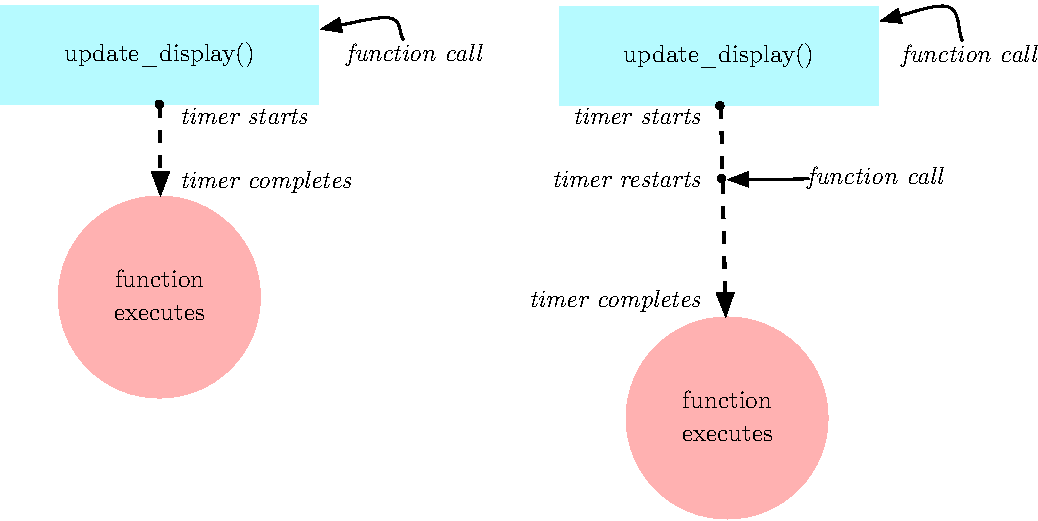
\includegraphics[width=1\textwidth]{figures/waiting_period}
		\caption{Illustration of a delayed function.}
		\label{fig:waiting_period}
\end{figure}

%Two functions are limited in the GUI: \url{view.update_display} for all views and \url{update_arrows} for ListView. \url{update_display} is common to all views, and the massive network changes described above can result in many processor intesive functions to run needlessly. With the \url{update_arrows} function, operations that do not result in changes to the network (scrolling, changing tabs) require constant re-drawing.

Exactly how much time this delay should be set to is not obvious. If the delay is too short it is possible for massive network operations to still cause multiple redundant display updates. A too-long delay means that users may perceive the delays for simple actions, like creating with a single arrow. Another consequence of a long delay is that a process which calls the delayed function at a regular interval could continuously restart the delay. In this case the function will \emph{never} execute, a situation known as ``starvation''.

After some informal tests of delays between 17 and 1000 milliseconds, a delay of 33 milliseconds was selected for both functions. Substantial improvement in execution speed was observed for even very short delays, as often hundreds of function calls would reach the \url{view.update_display} virtually simultaneously. With delays closer to one second we saw little improvement in response to massive network operations and the delay itself became noticeable. 33 milliseconds is in the range where nearly every operation results in a single function execution and is also imperceptible to a human user. The number 33 itself was selected because it is the length of two screen refreshes on a 60 Hz display (a measure recommended by \shortciteANP{os_concepts}).
	
	% subsection rate_limiting_certain_functions (end)

% section testing_program_responsiveness (end)

%%%%%%%%%%%%%%%%%%%%%%%%%%%%%%%%%%%%%%%%%%%%%%%%%%%%%%%%%%%%%%%%%%%%%%%%%%%%%%%%%%%%%%%%%%%%%%%%%%%%%%%%%%%%%%%%%%%%%%%%%%%%%%%%%%%%%%%%%%%%%%%%%%%%%%%%%%%%%%%%%%%%%%%%%%%%%%%%%%%%%%%%%%%%%%%%%%%%%%%%%%%%%%%%%%%%%%%%%%%%%%%%%%%%%%%%%%%%%%%%%%%%%%%%%%%%%%%%%%
\section{Comparison to Similar Interfaces} % (fold)
\label{sec:comparison_to_similar_interfaces}

Other systems exist to help non-programmers map control inputs to sound synthesis parameters. This section compares this research to these related works.

\begin{figure}[h]
	\centering
		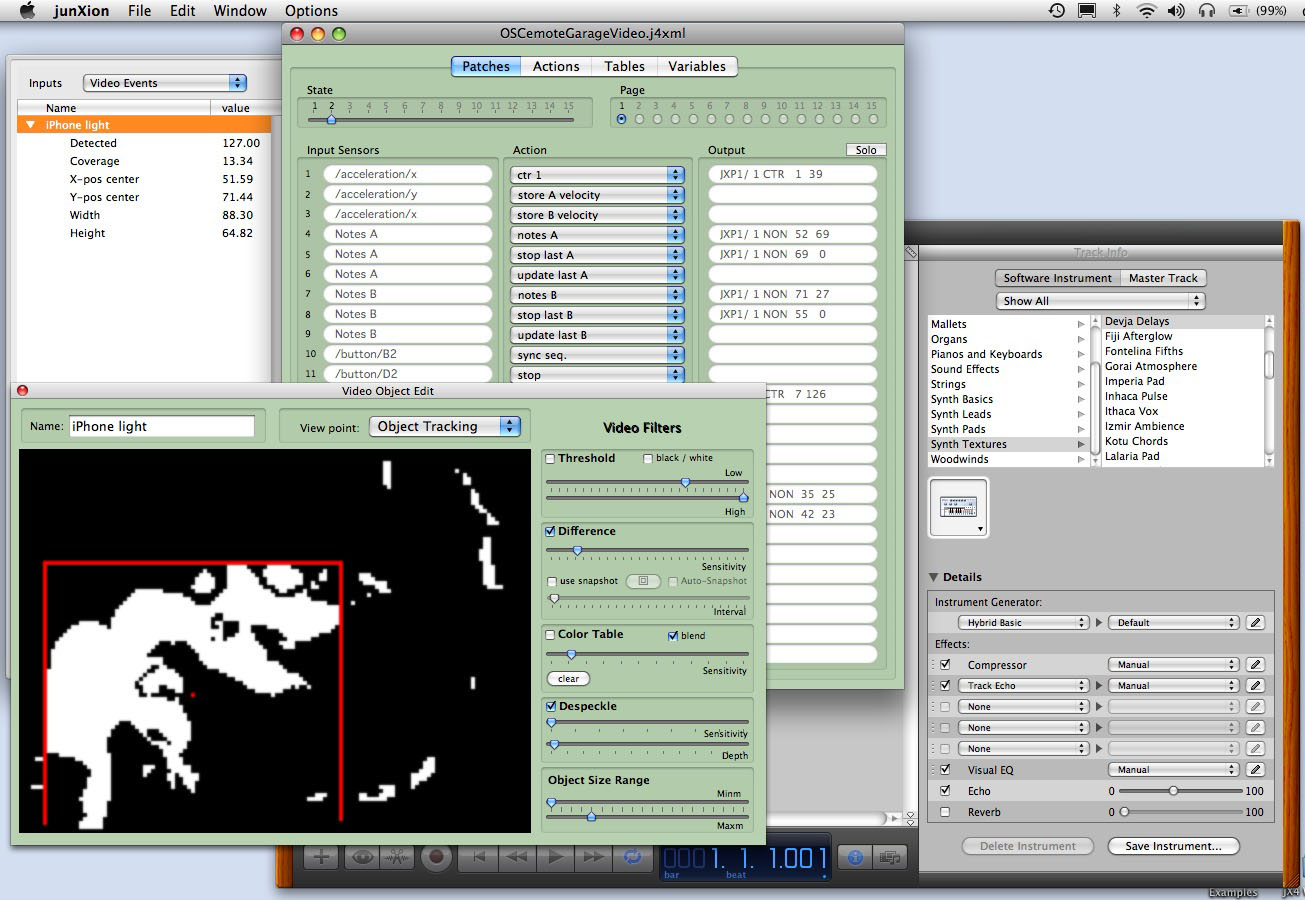
\includegraphics[width=\textwidth]{figures/junXion_v4}
		\caption{STEIM's JunXion software}
		\label{fig:junxion}
\end{figure}

The Studio for Electro-Instrumental Music (STEIM) distributes JunXion \cite{junxion}, a software application for controlling MIDI and OSC-based systems. JunXion automatically detects input devices like computer mice and USB video-game controllers. The user is able to drag child signals from these controllers onto one of 25 possible inputs.  From there users can switch to the ``actions'' tab, where destinations and connection properties are be customized. The program stores connection properties in groups that populate drop-down menus in the central column. JunXion features a very interesting ``state'' system similar to MapperGUI's saving and loading. Once a successful mapping is created, users can change the state, starting a new mapping. With multiple mappings, users can quickly switch between states. JunXion also has a very interesting graphical signal conditioning editor. The program presents a two dimensional field and the user can draw, generate curves and set bounds. Incorporating such a feature into MapperGUI would assist users who were unimpressed by textual expression input.

\begin{figure}[h]
	\centering
		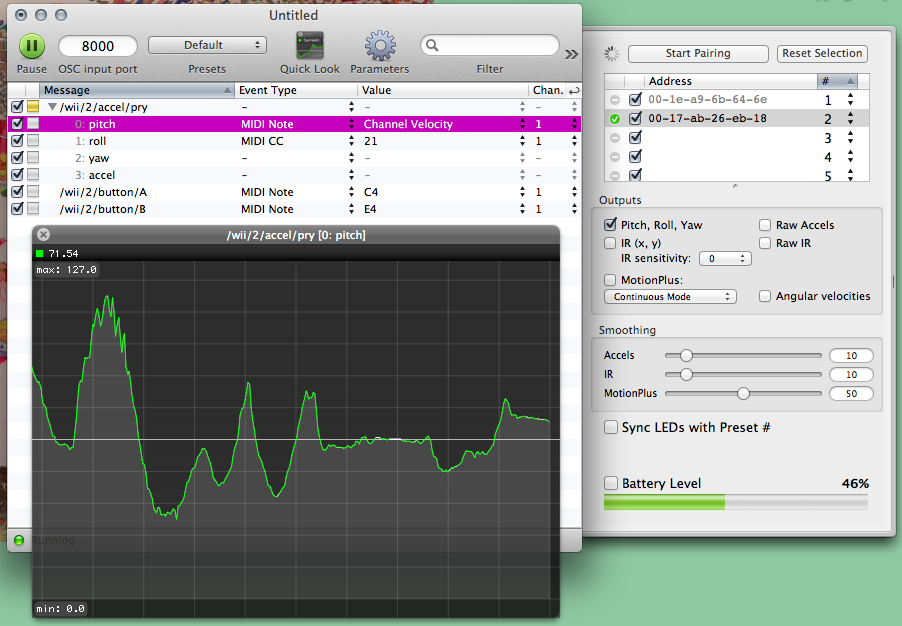
\includegraphics[width=\textwidth]{figures/osculator}
		\caption{The OSCulator interface}
		\label{fig:osculator}
\end{figure}

The OSCulator system \cite{osculator} is very similar to JunXion. Compatible controllers appear automatically and can be mapped to MIDI or OSC signals. OSCulator also relies on a drop-down menu based interface for selecting where and how the output will be routed. As in JunXion the idea of a ``connection'' is not emphasized, instead a MIDI or OSC message is simply sent on a specific channel (the receiving end must be notified on which channel to receive messages). As can be seen in Figure \ref{fig:osculator}, OSCulator displays a real-time oscilloscope-like visualization for selected signals. A similar feature would improve MapperGUI's with visual feedback, though require actual signal data from libmapper.

The Eaganmatrix \cite{eaganmatrix} partly inspired GridView in MapperGUI. The signals of a single control and synthesis device are displayed on the x and y axes of a grid display. Connections between the two are made by clicking on the intersections. The Patchage interface \cite{patchage} contains an interaction very similar to ListView: objects containing lists of signals can be connected by dragging gestures. Max/MSP and Integra Live \cite{integra} also feature this interaction, but neither are necessarily for creating mappings. 

	% subsection other_similar_interfaces (end)

% section comparison_to_similar_interfaces (end)

%%%%%%%%%%%%%%%%%%%%%%%%%%%%%%%%%%%%%%%%%%%%%%%%%%%%%%%%%%%%%%%%%%%%%%%%%%%%%%%%%%%%%%%%%%%%%%%%%%%%%%%%%%%%%%%%%%%%%%%%%%%%%%%%%%%%%%%%%%%%%%%%%%%%%%%%%%%%%%%%%%%%%%%%%%%%%%%%%%%%%%%%%%%%%%%%%%%%%%%%%%%%%%%%%%%%%%%%%%%%%%%%%%%%%%%%%%%%%%%%%%%%%%%%%%%%%%%%%%
\section{Evaluation of Goals} % (fold)
\label{sec:evaluation_of_goals}

A set of goals for the software was established at the beginning of this document. These were to create an interface for libmapper that was easy to use for non-programmers and to make this interface modular and multi-platform. Of primary concern was to create a system that was flexible and intuitive. We also intended to unite features of the three prior GUIs, both to capitalize on work already completed and to create a single, standard graphical interface for libmapper. 

Our GUI currently exists in a distributable form, allowing Macintosh users to download and easily use the software. Unfortunately standalone applications for non-Macintosh platforms are not yet available. Most features from prior interfaces were integrated into a cross-compatible web-based system. A modular code-base was created for the application, greatly improving the processes of maintaining and extending this GUI verses prior interfaces. Two new view modes were integrated into the display, though it is too early to conclude as to whether they significantly contribute to the flexibility of the system.

The software was provided to users, and thus tested in a variety of contexts. MapperGUI was able to handle most use-cases in its present state. All shortcomings were recorded, those that have not yet been addressed are listed along with possible solutions in Section \ref{sec:future_work}. Though it has not yet been the case, in the future MapperGUI will likely be used to handle mappings in a live performance context. This will give us a new perspective on how the software performs in a situation where instant reactivity is a necessity and errors can be disastrous. 
	
% section evaluation_of_goals (end)





%
\typeout{}
%!TEX root = ../thesis.tex
\chapter{Conclusions \& Future Work}

This chapter summarizes the work presented this thesis, presents conclusions, and summarizes possible avenues for further research.

\section{Summary and Conclusions}

This thesis began by exploring issues relevant to musical mapping interfaces. DMI designers typically hard-code mappings into their designs, making collaboration, cross-compatibility and modification difficult. Certain tools exist to aid these designers and their users, but often they are difficult to use for non-experts in computer programming. Our work was motivated by this situation in musical mapping software. MapperGUI aimed to lower the barriers to entry for those who wished to use libmapper, a software library for collaborative and configurable musical mapping. The GUI was designed to allow for quick and straightforward manipulation of musical networks. 

Techniques from data visualization and user interface design were presented to illustrate general principles used in MapperGUI's design. The ideas and structure of libmapper were summarized to describe the requirements of a GUI for the library. Prior GUIs for libmapper were described, as ideas and code were borrowed from them in the creation of MapperGUI.

The final GUI took the form of a modular interface. Various independent view modes could be swapped in and out by the user, making MapperGUI useful for a wider variety of libmapper networks. The code itself was also structured in a modular fashion such that extensions could be created more easily. The program was made accessible to libmapper users throughout this project, and their feedback became a crucial factor in design decisions. 

MapperGUI has met many of the goals set at the beginning of this thesis work. The interface is available, functional and very accessible. The majority of libmapper variables can be accessed and manipulated from within the GUI. Within ListView connection and linking are easy and intuitive. Two alternate views are present for networks and tasks where list-type views are cumbersome. Users can save and load mappings.

The current release of MapperGUI, however, is still in a test phase. A number of issues need to be resolved before the software can be adopted as standard GUI for libmapper. 

\section{Future Work}

	\subsection{Unimplemented features}

A few features present in Maxmapper have not yet been implemented in MapperGUI. Most importantly, MapperGUI currently does not support sending a signal as an instance. Instances are one of the true strengths of libmapper. To design a way, even an inelegant way, to allow the user to take advantage of this libmapper feature is a high priority for the next release. Users are also unable to edit link scopes in the current version. Support for this will be fairly easy to implement, via a drop-down menu on the top bar and some extensions to the python monitor. 

Our search functions, though usable, are not yet quite as powerful as those found in Maxmapper. Maxmapper allows users to filter signals for common prefixes, by way of a drop-down menu.  MapperGUI also forces users to remain on whichever network on which the program was launched. In the case where multiple networks are available, it would be a good extension to allow users to select and switch between them. Finally, MapperGUI's expression editing was poorly reviewed by users. Upon a double click of the \emph{Expression} button, Maxmapper displays a palate with all possible expression syntax (to create exponential functions, averages, etc.). Incorporating this feature would be a good start.

%	\begin{enumerate}
	%	\item Prefix filtering
	%	\item Network selection
	%	\item Expression Palate 
	%	\item Edit scopes
	%	\item Send as instance
%	\end{enumerate}

	\subsection{Possible extensions} % (fold)
	\label{sub:possible_extensions}

With the MVC architecture and some alternate views in place, our group has planned extensions to MapperGUI that may be very interesting. Firstly, HiveView should be made fully interactive, allowing the user to create links and connections with a dragging gesture. The hierarchical edge bundling technique described in Section \ref{sec:color} would be very useful for this view, as currently connection lines are drawn somewhat arbitrarily. Attempts were made to integrate Vizmapper into MapperGUI as a single view, as it was an initial goal of the process. Unfortunately idiosyncrasies in the Vizmapper code-base made this more difficult than anticipated. In the future the we hope to restructure the Vizmapper code so that it might be included, as it is a very interesting and effective network visualization. 

Another way that the research in Section \ref{sec:color} could be applied is through a new ``area'' view mode. In this mode network elements would be displayed as shapes on a Cartesian plane, with each axis user-mappable to any kind of quantitative metadata. Other metadata could be visually mapped to these shapes' color, orientation, shape, opacity, etc. This would be a very interesting way to analyze the findings of \citeN{visual_dimensions}, and may be the topic of a future project. 

The saving and loading features of MapperGUI obviously need improvement. Work has already begun on a staging process for loaded mappings, such that saved mappings are only loaded for the desired devices. Finally, standalone support for Windows and Linux systems is definitely required for future releases of MapperGUI. It would also be interesting to begin work on mobile versions of MapperGUI, though that would be a much more time-consuming process. 

	%\begin{enumerate}
		%\item HEB for hive
		%\item Integrate vizmapper
		%\item Save/Loading Rehaul
		%\item Standalone for Windows and Linux
		%\item Mobile support
		%\item Area view to make good on variable analysis
	%\end{enumerate}
	% subsection possible_extensions (end)


	
%%==========



%%========== Appendices
%\appendix
%
%%==========
%\typeout{}
%\input{A-A}

%========== Bibliography
\typeout{}
%\begin{singlespace}
    \renewcommand\refname{References}
    \bibliography{../citations/references,../citations/other_references}
    \bibliographystyle{Style/ichago}
%\end{singlespace}

\end{document}
